% \documentclass{ifacconf}

% \usepackage{graphicx}
% \usepackage{url} 
% \usepackage{amsmath,amssymb,amsfonts}
% \usepackage{algorithm}
% \usepackage{algpseudocode}
% \usepackage{balance}

% \usepackage{natbib}

\documentclass{ifacconf}

\usepackage{graphicx}
% \usepackage{url} % 注释掉原本的 url
\usepackage{xurl}  % 使用 xurl 代替，完美解决长链接换行问题
\usepackage{amsmath,amssymb,amsfonts}
\usepackage{algorithm}
\usepackage{algpseudocode}
\usepackage{balance}
\usepackage{natbib}

% 将 hyperref 放在最后
\usepackage[bookmarks=false, hidelinks]{hyperref}

\begin{document}
\begin{frontmatter}

\title{Control of Mixed-Autonomy Traffic via Autonomous Vehicles with Lane-Changing Behavior}

\thanks[footnoteinfo]{This work was supported by the Holland High Tech (TKI HTSM) strategic program PPS-I Flex HighTech under the project number 24PPS173-CABS.}




\author[NL]{Shuwei Pei} 
\author[TK]{Muhammed O. Sayin}
\author[NL]{Saeed Ahmed} 

\address[NL]{Engineering and Technology institute Groningen, Faculty of Science and Engineering, University of Groningen, 9747 AG Groningen, the Netherlands (e-mails: s.pei@rug.nl, s.ahmed@rug.nl)}
\address[TK]{Department of Electrical, Electronics Engineering, Bilkent University, TR-06800 Ankara, Turkey (e-mail: sayin@ee.bilkent.edu.tr)}

\begin{abstract}                
Recent work \citep{9765650} showed that a single autonomous vehicle (AV) can stabilize stop-and-go oscillations on a double-lane ring road, assuming human drivers do not change lanes. We discovered that extending this paradigm to a single AV trained with human lane-changing is insufficient: it still fails to stabilize traffic flow. Motivated by this, we study a double-lane ring road with human lane-changing and propose a rule-based, pair-aligned control strategy via two AVs that synchronizes their motion across lanes. This controller suppresses human lane-changing, couples the two lanes into a single virtual lane, and mitigates oscillations. Its structure is inspired by cooperative reinforcement learning (RL) experiments, where two AVs repeatedly learned to form a cross-lane paired configuration. In simulations, our controller increases stabilized average speed by 7.4\% compared to two AVs equipped with a single-lane stabilization controller \citep{9765650}.
\end{abstract}

\begin{keyword}
Traffic control, connected AVs, RL, intelligent transportation systems
\end{keyword}

\end{frontmatter}

\section{Introduction}
Stop-and-go traffic waves on highways have emerged as a critical challenge, contributing to travel delays, collision risk, and environmental impact \citep{laval2010mechanism}. The integration of AVs into road networks introduces new opportunities for intelligent traffic management.  
More recently, learning-based approaches in AVs have gained prominence, particularly in RL. These methods learn control policies directly from interaction data, enabling AVs to handle the unpredictability of human-driven vehicles (HDVs). Applications range from bottleneck \citep{vinitsky2020optimizing} and merging scenarios \citep{liu2021efficient} to stop-and-go wave suppression \citep{wu2018stabilizing,9765650} and network-level coordination \citep{suriyarachchi2022multi}. 
  
From a methodological perspective, existing traffic control studies fall into three groups: rule-based, optimization-based, and learning-based methods. Rule-based approaches manage traffic through predefined policies or heuristics, favored for simplicity and interpretability. For instance, adaptive cruise control (ACC) mitigates oscillations using distance and speed feedback \citep{vahidi2004research}, while cooperative ACC (CACC) enhances stability via tighter coordination \citep{van2006impact}. 

Optimization-based methods formulate explicit optimization problems grounded in vehicle and network dynamics. \citet{newell2002simplified} introduced a widely adopted car-following model, while the intelligent driver model (IDM) \citep{treiber2000congested} remains highly influential. Building on these, robust control \citep{zheng2020smoothing} and model predictive control (MPC) \citep{feng2021robust} have emerged to handle constraints and multiple objectives. However, solving constrained optimizations continuously introduces significant computational burdens. 
\begin{figure}[t!]
    \centering
    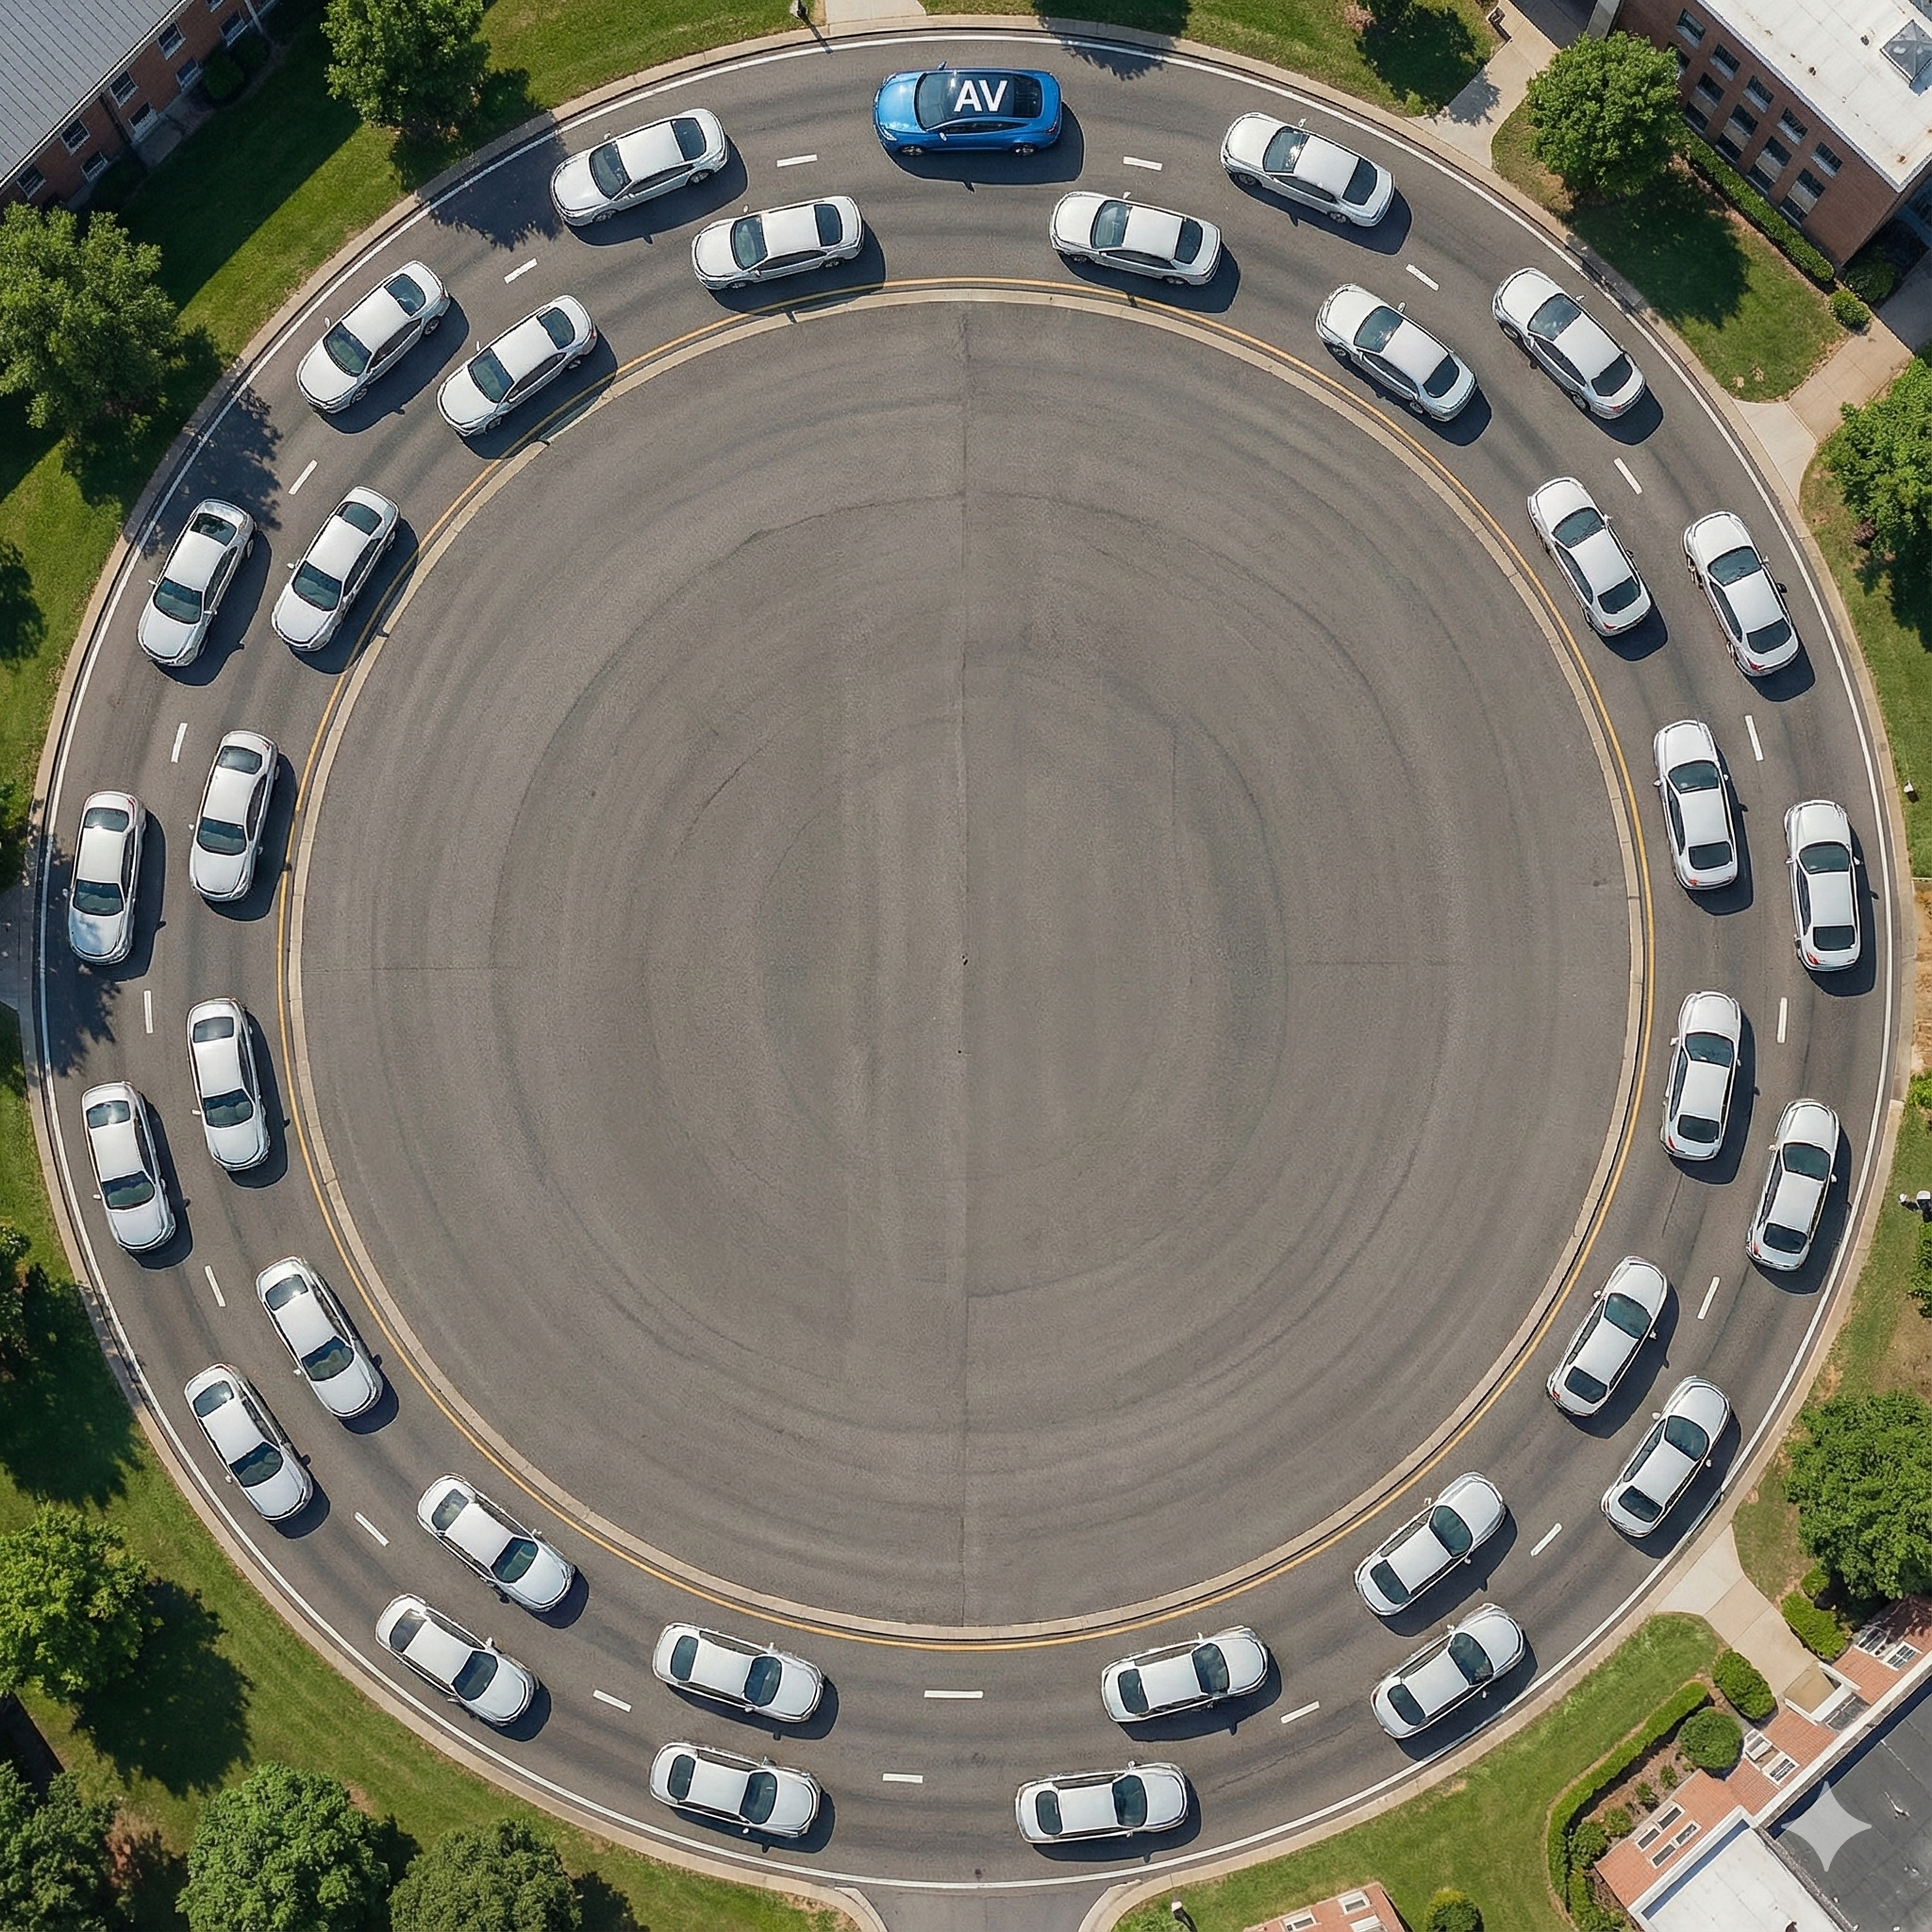
\includegraphics[width=0.6\linewidth]{doublelaneringnetwork_2.png}
    \caption{Double-lane ring road. 
The blue vehicle denotes an AV, while the remaining vehicles represent HDVs.}
    \label{fig:Network}
\end{figure}
Recently, learning-based methods have attracted growing attention for traffic management. Unlike rule- or optimization-based approaches, they can directly learn policies from data and driving behaviors with improved computational efficiency. \citet{wu2018stabilizing} demonstrated that structured rule-based control strategies can be extracted from the emergent behaviors of RL-controlled AVs in ring road settings. Subsequent work explored platoon-based control \citep{shi2023deep}, multi-agent coordination with shared policies \citep{suriyarachchi2022multi}.
Nevertheless, most studies focus on longitudinal control, often neglecting unpredictable human lane-changing in mixed traffic. While \citet{9765650} showed a controller derived from RL can stabilize a double-lane ring road (Fig.~\ref{fig:Network}) without HDV lane changes, it remains unclear if this holds with realistic lane-changing. This study addresses this open question. 
 
Through simulations, we first evaluated a single RL-controlled AV in this unpredictable setting. The AV learned to aggressively minimize headways to suppress HDV lane changes, yet stop-and-go oscillations persisted. Building on this, we extended the framework to two cooperative RL-controlled AVs with a shared reward encouraging coordination. This mitigated oscillations and revealed an emergent pattern: the AVs naturally formed a cross-lane paired structure. Based on this, we derive a rule-based pair-aligned controller (Fig.~\ref{fig:overview}) that explicitly enforces this formation. It synchronizes the AVs, suppresses lane changes, and effectively couples both lanes into a single virtual lane, achieving high average speed.

\begin{figure}[t!]
    \centering
    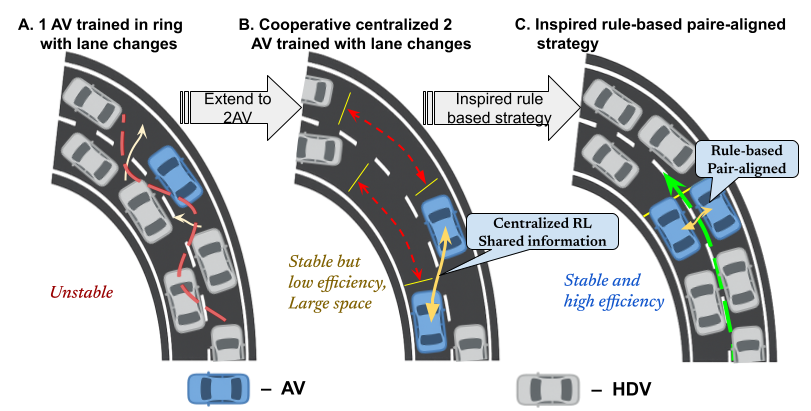
\includegraphics[width=1\linewidth]{The overview of paired controller for stabilizing flow.png}
    \caption{Paired-controller design. A single AV fails to suppress oscillations (left). Two cooperative AVs form a stable but conservative pattern, limiting efficiency (middle). The proposed rule-based controller coordinates the AVs, suppresses disruptive lane changes, and achieves stability and high efficiency (right).}
    \label{fig:overview}
\end{figure}

{\it Contribution:}

\begin{enumerate}
    \item We developed cooperative RL for two AVs, which naturally yields an emergent cross-lane paired formation that suppresses oscillations and human lane-changing.
    \item Inspired by this, we designed a rule-based pair-aligned controller that couples both lanes into a virtual lane, preventing HDV lane changes. It improves stabilized average speed by 7.4\% compared to using two independent single-lane controllers.

\end{enumerate}

{\it Organization:} Section~\ref{PDSGO} formulates the problem. Section~\ref{sec:Single} evaluates a single RL AV. Section~\ref{sec:Cooperative} investigates cooperative RL and the emergent paired formation. Section~\ref{sec:pair} introduces our rule-based controller. Section~\ref{sec:Discussion} compares approaches, and Section~\ref{sec:Conclusion} concludes.

\section{Problem Formulation}\label{PDSGO}

Stop-and-go traffic is characterized by repeated deceleration–acceleration cycles. We investigate this in a double-lane ring road simulation, where human lane-changing and heterogeneous driving behaviors induce persistent oscillations (Fig.~\ref{fig:stop-and-go}). While prior work \citep{9765650} demonstrated stop-and-go mitigation via a single AV in a double-lane ring, it unrealistically restricted human drivers from changing lanes. We relax this assumption to model realistic mixed traffic.

\begin{figure}[t!]
    \centering
    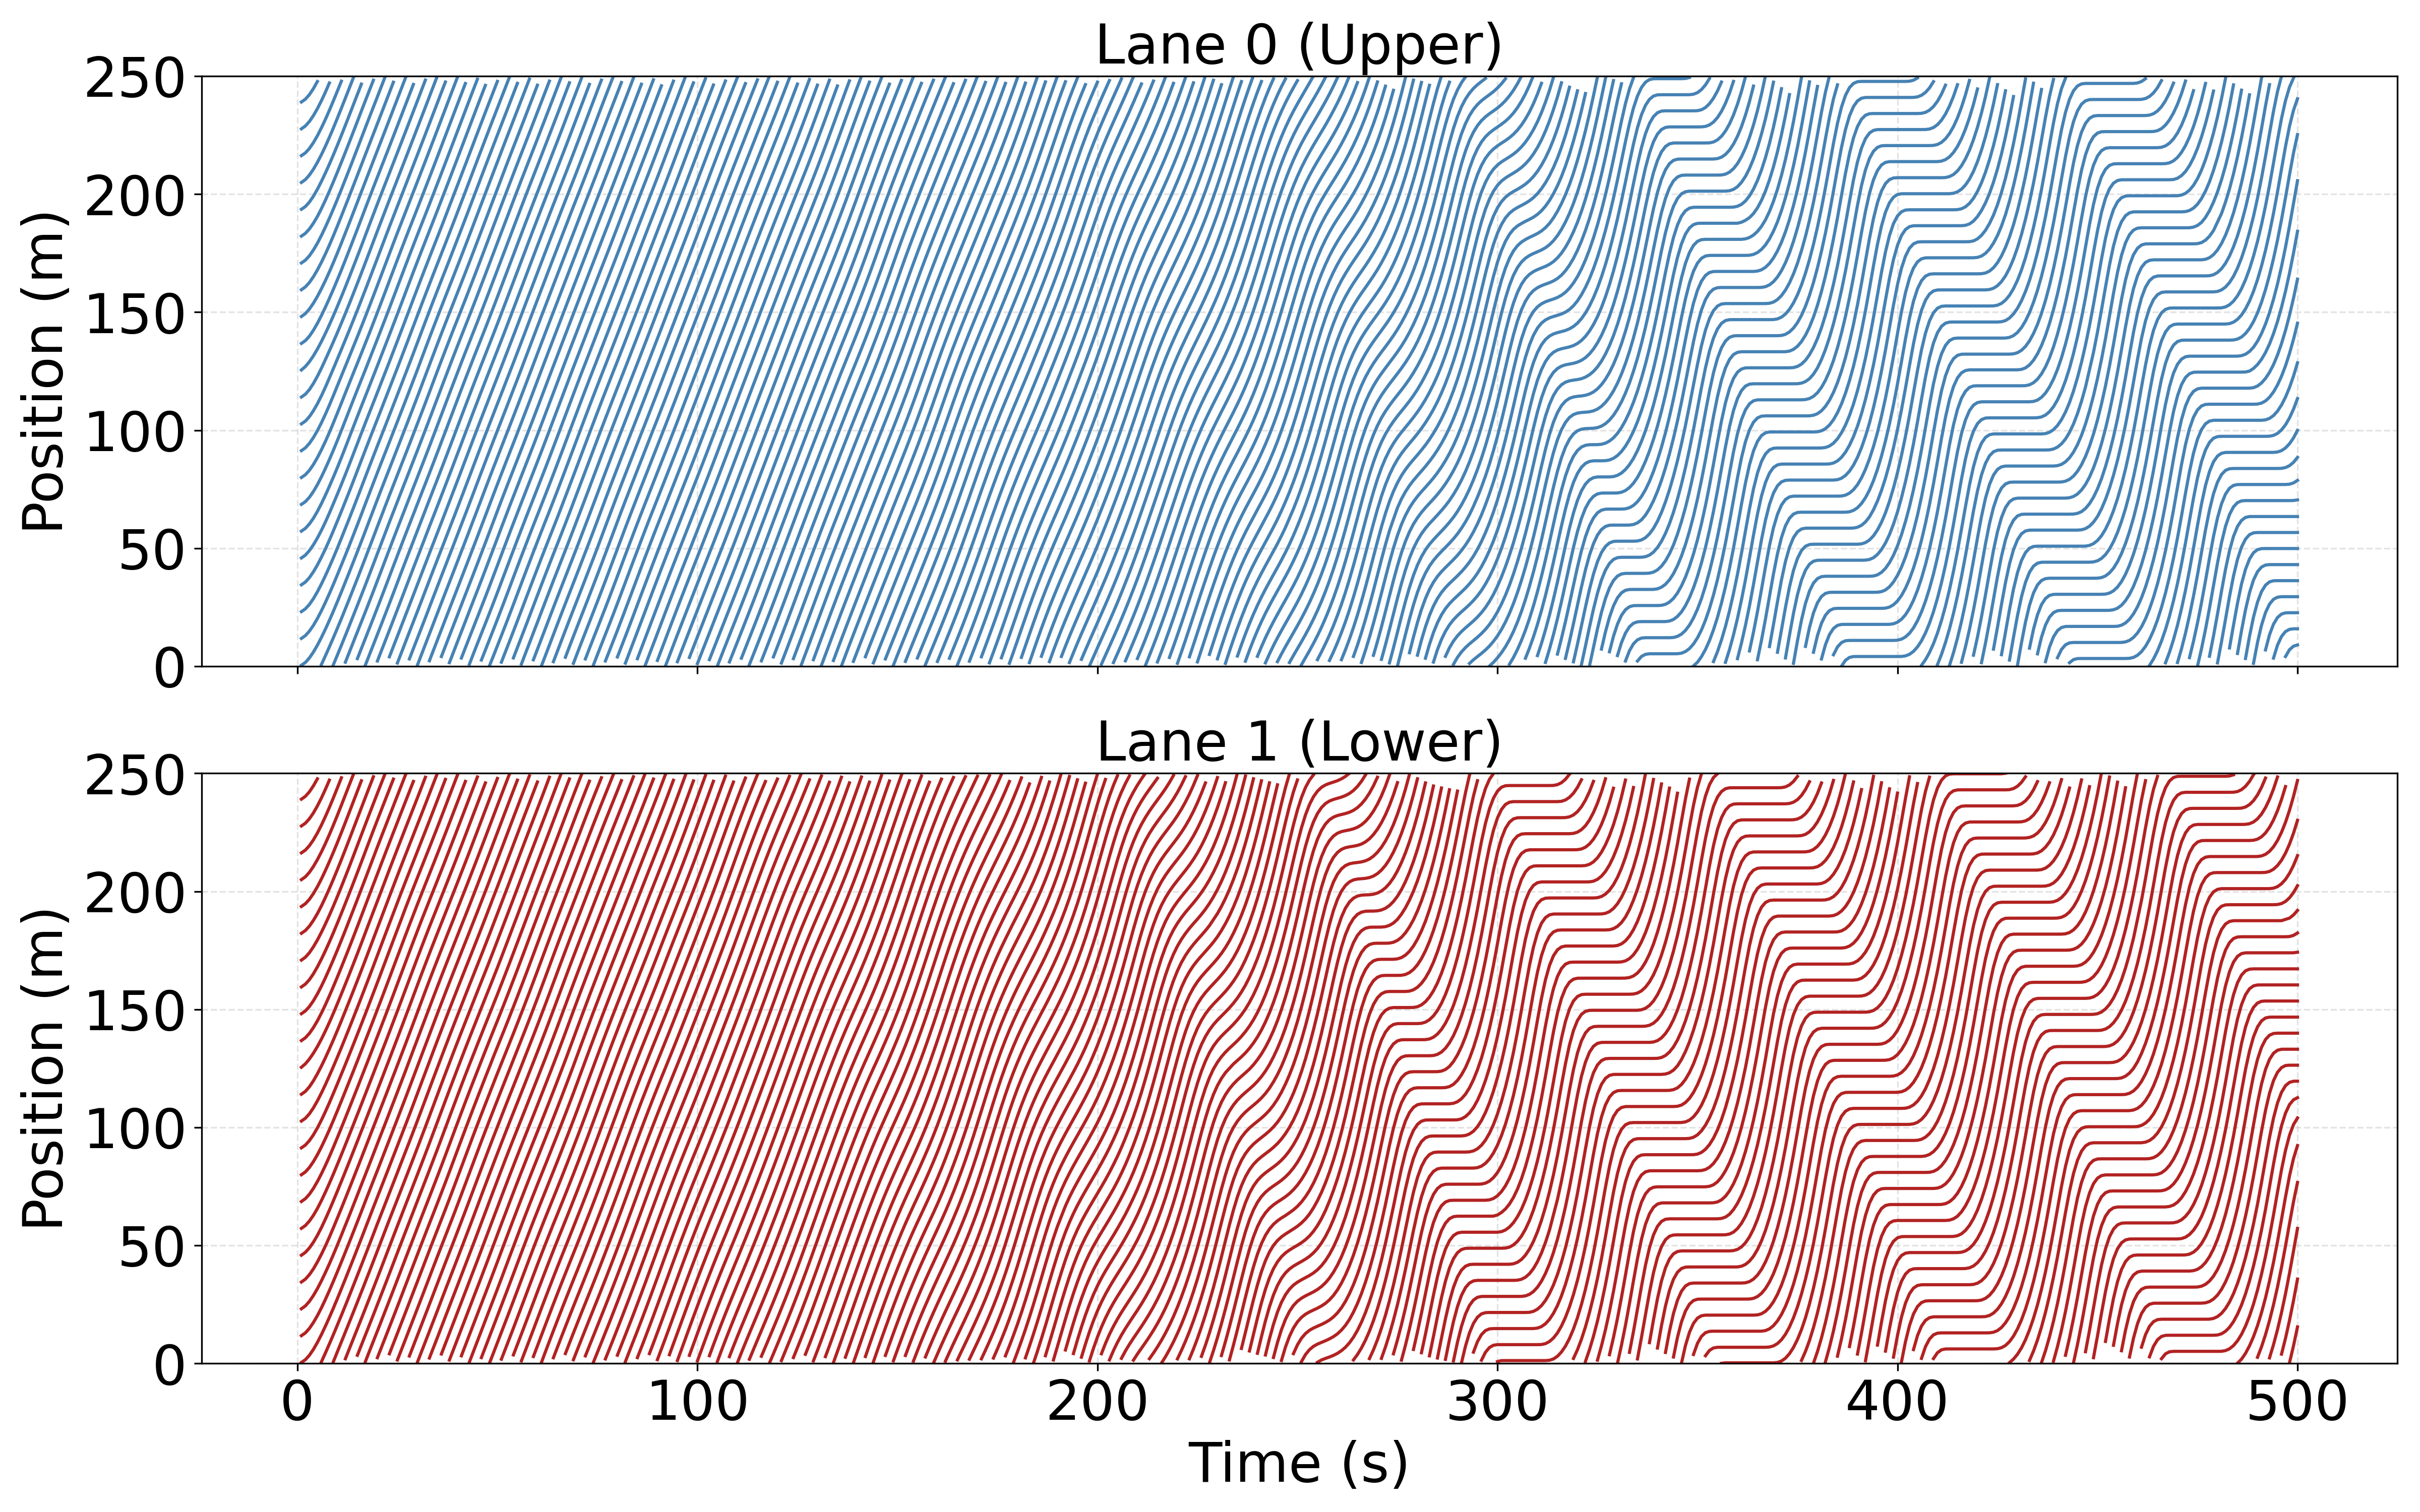
\includegraphics[width=1\linewidth]{trajectory_log_allhuman44.png}
    \caption{Stop-and-Go oscillations.}
    \label{fig:stop-and-go}
\end{figure}

\subsection{Formulation as an RL Problem}
\label{subsec:rl_formulation}

We model vehicular control as a finite-horizon discounted Markov Decision Process (MDP) \citep{puterman2014markov}, defined by the tuple $\mathcal{M} = (\mathcal{S}, \mathcal{A}, \mathcal{T}, r, \rho_0, \gamma, H)$. Here, $\mathcal{S}$ and $\mathcal{A}$ are the state and action spaces. The transition kernel $\mathcal{T}(s' \mid s, a)$ governs stochastic dynamics, $r(s, a, s')$ defines the reward, $\rho_0$ is the initial state distribution, $\gamma \in [0,1)$ is the discount factor, and $H$ is the horizon. 

The objective is to learn a policy $\pi(a \mid s)$ maximizing the expected return \citep{sutton1998reinforcement}:
\begin{equation*}
\max_{\pi} J(\pi) = \mathbb{E}_{\pi} \left[ \sum_{t=0}^{H-1} \gamma^t r(s_t, a_t, s_{t+1}) \right].
\label{eq:mdp_objective}
\end{equation*}

For our double-lane mixed traffic environment:
\begin{itemize}
    \item \textbf{State space $\mathcal{S}$}: Local observations (e.g., relative speeds/distances to neighbors) and shared variables (e.g., AV positions/velocities).
    \item \textbf{Action space $\mathcal{A}$}: AV acceleration and lane-changing decisions.
    \item \textbf{Reward $r$}: Designed to maximize average speed and AV synchronization while penalizing aggressive acceleration.
\end{itemize}

These components are formalized subsequently. We begin with a single-agent setting (one AV among human-driven vehicles) and extend to cooperative multi-agent RL, where enriched state observations and cooperative rewards promote system-level efficiency. 


\subsection{Simulation Setup}
Simulations are conducted in SUMO using Flow \citep{wu2017flow} on a 250\,m double-lane ring road with 44 vehicles. A 500\,s warm-up period induces stop-and-go oscillations, where all vehicles act as IDM \citep{treiber2000congested} and randomized LC2013 \citep{erdmann2015sumo} drivers to generate realistic, unpredictable human lane changes. The AV is governed by an MLP-based RL policy. The source code for our simulations and proposed controllers is publicly available at \url{https://github.com/TravidP/RL_Inspired_Controller_of_Mixed_Traffic_Lanechanging}. 
 
\section{Single-Agent Reinforcement Learning}\label{sec:Single}
We first deploy a single RL-controlled AV among lane-changing HDVs.

\subsection{Observation, Action, and Environment Specification}
The observation vector $o_t \in \mathbb{R}^{11}$ captures the AV's normalized speed and, for each lane $\ell \in \{0,1\}$, a lane indicator and the normalized relative distance and speed of its immediate leader and follower:
\begin{equation*}
o_t = \Big[ \tfrac{v_t^{AV}}{v_{\max}}, \; \mathbf{z}_{t}^{(0)}, \; \mathbf{z}_{t}^{(1)} \Big], \;
\mathbf{z}_{t}^{\ell} = \Big[ \mathbf{1}_{\{\ell = \ell_t\}}, \tfrac{d_{f,t}^{\ell}}{L}, \tfrac{v_{f,t}^{\ell}}{v_{\max}}, \tfrac{d_{b,t}^{\ell}}{L}, \tfrac{v_{b,t}^{\ell}}{v_{\max}} \Big].
\end{equation*}
The action $a_t$ comprises a continuous longitudinal acceleration $a^{\text{acc}}_t \in [-0.5, 0.5]$ and a lane-changing command mapped to $\{-1,0,+1\}$ via a threshold $\delta=0.33$.

\subsection{Reward Design}
The AV receives a reward equal to the instantaneous average speed of all vehicles, encouraging system-wide traffic efficiency.

\subsection{Results and Analysis}
As shown in Fig.~\ref{fig:1AVLC}, stop-and-go oscillations persist. The AV learns to maintain a tight headway to its leader, minimizing gaps to suppress HDV lane changes, which act as strong disturbances causing sudden braking and propagating waves. 
However, this locally optimal strategy merely prevents the AV from being trapped behind merging HDVs, without resolving overall traffic instability. These results underscore that human lane-changing is a primary destabilizing factor, motivating the need for cooperative multi-AV strategies to jointly suppress lane changes and enhance stability.
\begin{figure}[t!]
    \centering
    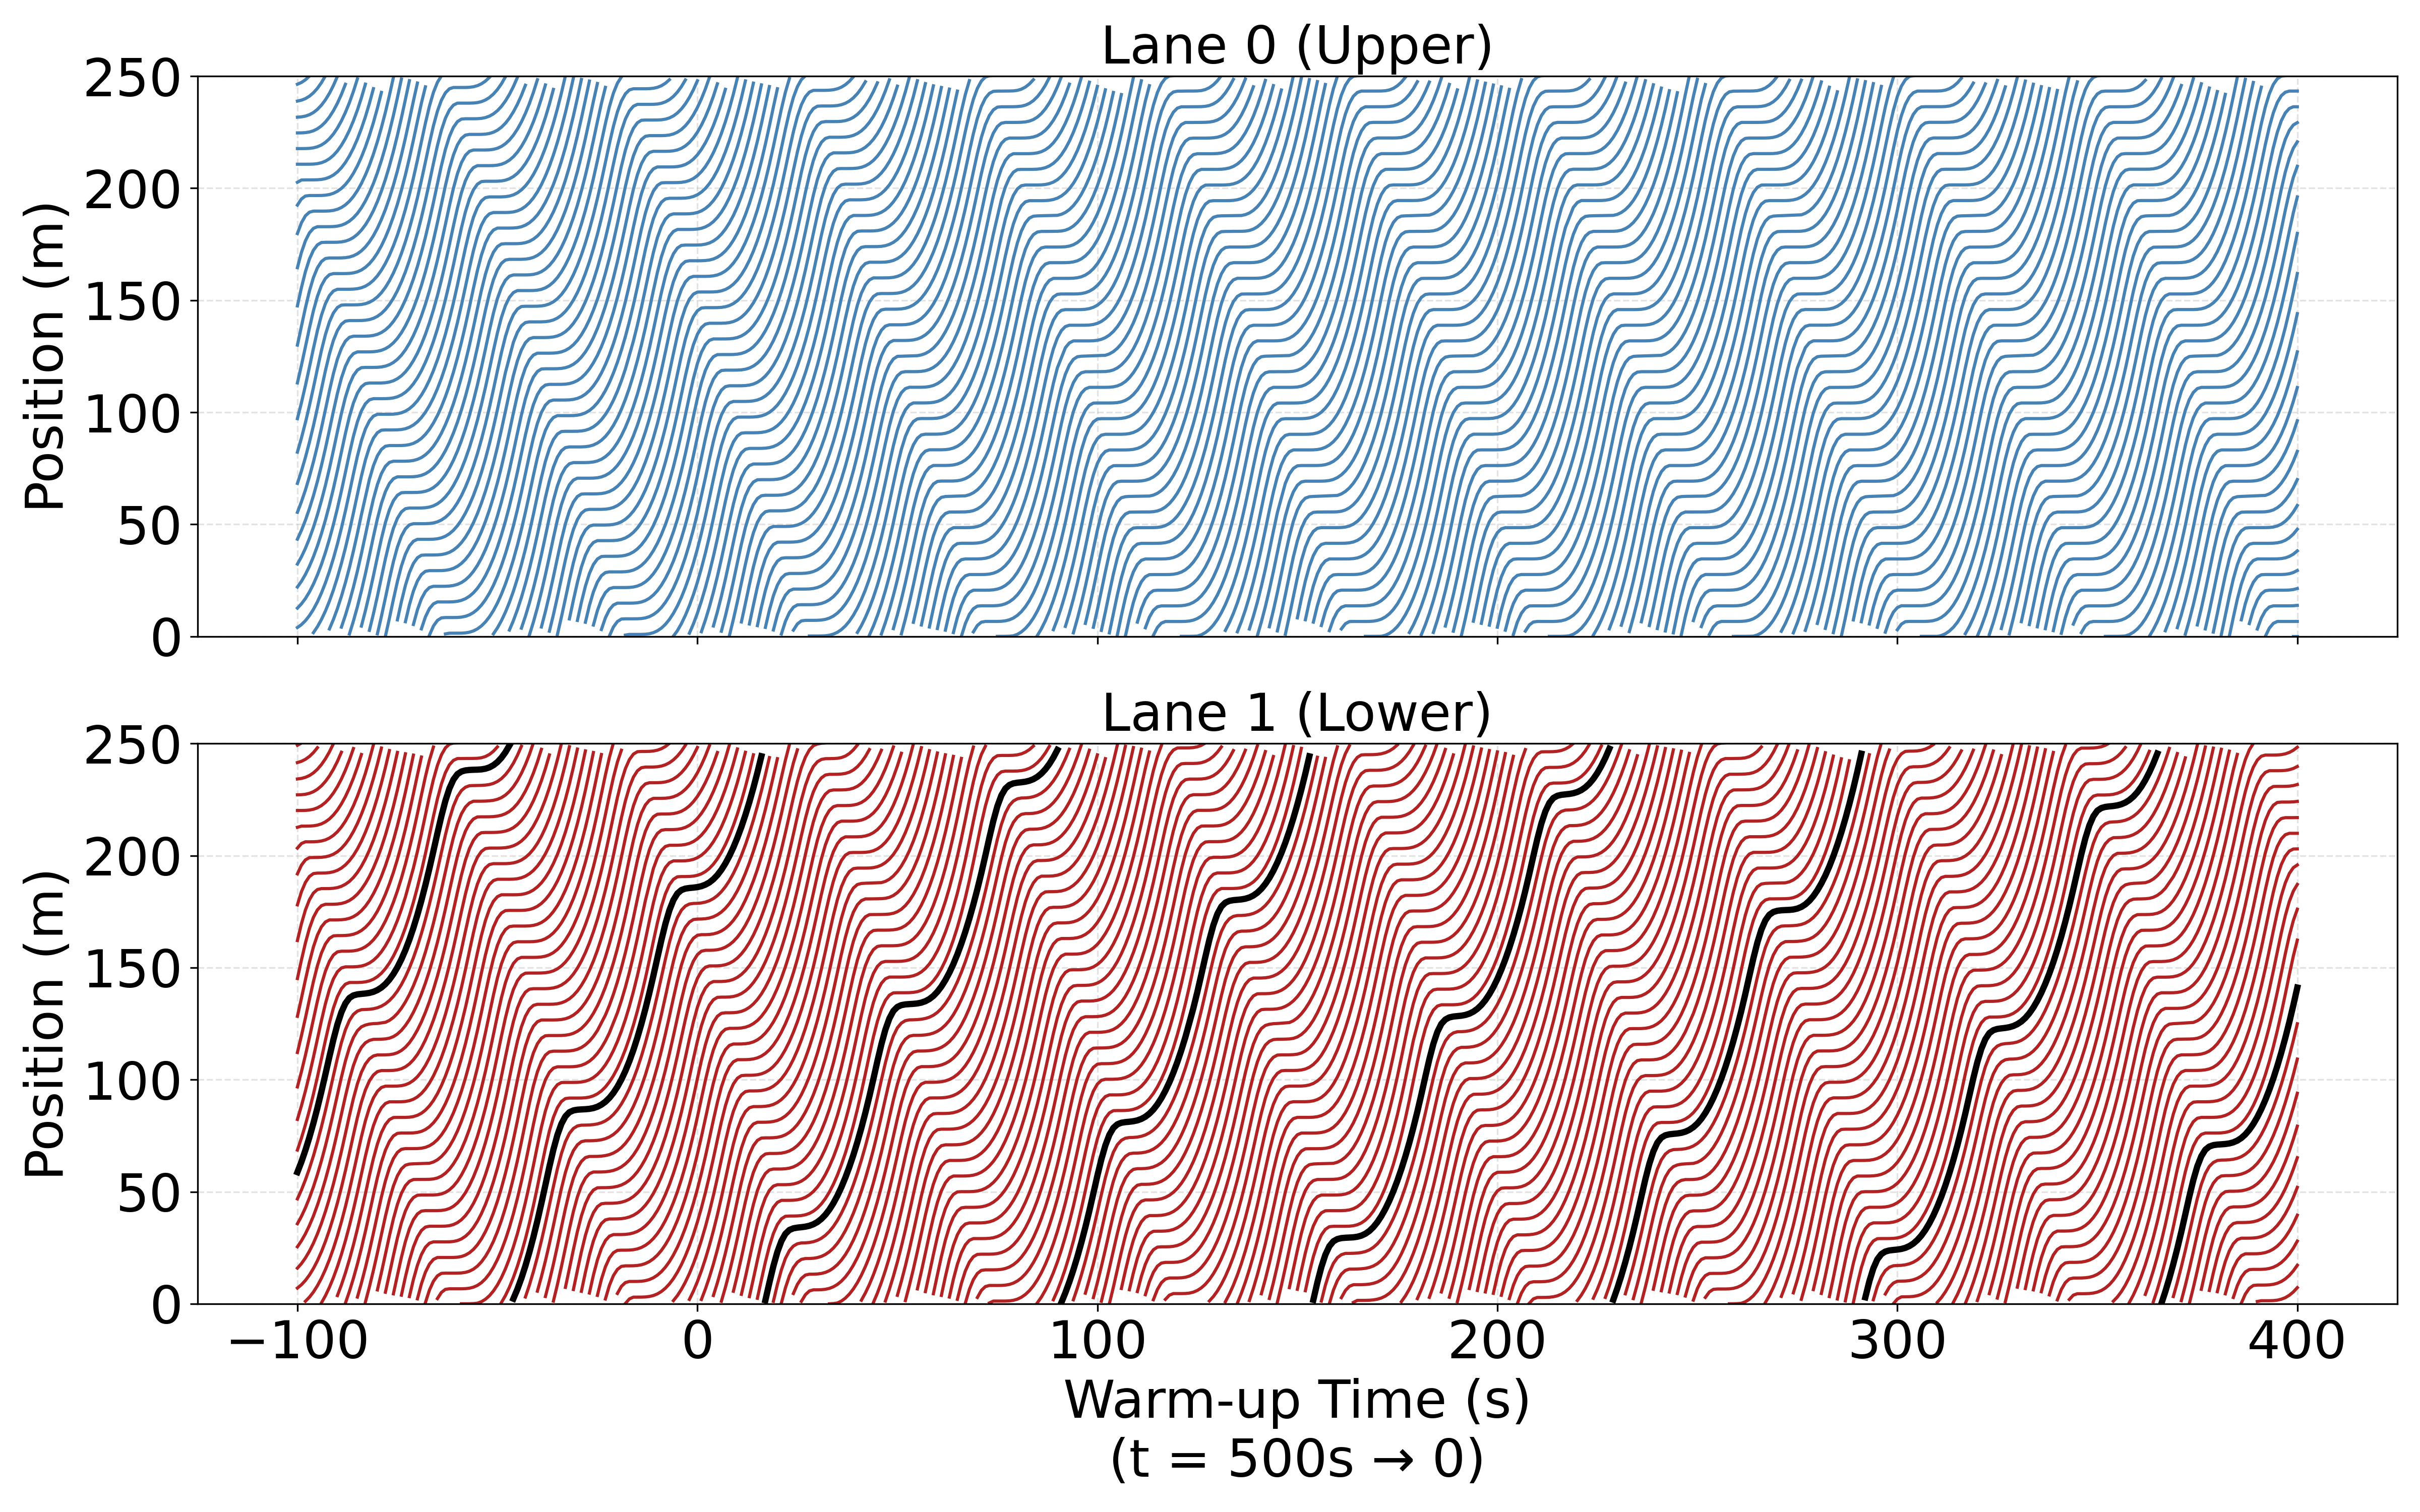
\includegraphics[width=1\linewidth]{trajectory_log_1AVLC.png}
    \caption{Time space diagram: Single-agent RL controller with one AV in a double-lane ring road with lane-changing HDVs.}
    \label{fig:1AVLC}
\end{figure}

\section{Cooperative Reinforcement Learning}
\label{sec:Cooperative}
We deploy a shared RL policy governing two AVs. To suppress unnecessary lane changes, both AVs are restricted to their assigned lanes, focusing exclusively on longitudinal control.

\subsection{Observation, Action, and Environment Specification}
The agent receives centralized continuous observation that captures relevant lane-level traffic features and pairwise coordination information. The observation vector has dimension $12$ and includes, for each AV: its own velocity, the velocity and gap of its lane leader and follower, as well as two cooperative terms representing the signed longitudinal distance and relative velocity between the two AVs. 
At each time step $t$, the $i$th AV $i \in \{1,2\}$, receives a lane-local observation vector:
\begin{equation*}
o^{i}_{t} =
\Big[
    \tfrac{v_t^i}{v_{\max}},\;
    \tfrac{v^{\mathrm{lead}}_{i,t}}{v_{\max}},\;
    \tfrac{v^{\mathrm{foll}}_{i,t}}{v_{\max}},\;
    \tfrac{d^{\mathrm{lead}}_{i,t}}{L},\;
    \tfrac{d^{\mathrm{foll}}_{i,t}}{L}
\Big],
\end{equation*}
where $v_t^i$ is the speed of the $i$th AV, 
$v^{\mathrm{lead}}_{i,t}$ and $v^{\mathrm{foll}}_{i,t}$ denote the speeds of the lane leader and follower,
and $d^{\mathrm{lead}}_{i,t}$ and $d^{\mathrm{foll}}_{i,t}$ are the corresponding headways.  
All speeds are normalized by $v_{\max}$ and all distances by the ring length $L$. Here, index $i \in \{1,2\}$ refers to the relative ordering of the two AVs
along the ring: AV~1 is the front vehicle, and AV~2 is the back 
vehicle. This ordering is updated at each time step.

To capture inter-lane cooperative behavior between the two AVs, two additional pairwise states are included:
\begin{equation*}
\left[
d_{\mathrm{AV},t},\;
\Delta v_{\mathrm{AV},t}
\right]
=
\left[
\frac{x_t^1 - x_t^2}{L},\;
\frac{v_t^1 - v_t^2}{v_{\max}}
\right].
\end{equation*}
where $x_t^1$ and $x_t^2$ are the positions of the AVs in the double-lane ring network.

Stacking the lane-local and cooperative components gives the complete observation vector:
\begin{equation*}
o_t = 
\big[
    o^{1}_t,\;
    o^{2}_t,\;
    d_{\mathrm{AV},t},\;
    \Delta v_{\mathrm{AV},t}
\big]
\in \mathbb{R}^{12}.
\end{equation*}

The action applied at time $t$ consists of continuous longitudinal accelerations for the two AVs:
\begin{equation*}
a_t
=
\begin{bmatrix}
a_1(t) \\
a_2(t)
\end{bmatrix}
\in 
\big[-0.5,\, 0.5\big]^2,
\end{equation*}
where $a_{i,t}$ is the commanded acceleration of the $i$th AV, bounded by acceleration and deceleration limits.

\subsection{Reward Design}

At each time step $t$, the centralized reward function encourages the two AVs to jointly maintain a stable formation, reduce unnecessary gaps, synchronize speeds, and maximize traffic throughput while ensuring smooth control. 
The reward consists of four components:
\begin{align*}
r_{\mathrm{pos},t} &\!=\! 
    -w_{\mathrm{pos}}
    \left|
        \frac{x^1_t - x^2_t}{L}
    \right|,\;\; r_{\mathrm{smooth},t} \!=\! 
    -w_{\mathrm{smooth}}
    \alpha_t,\\
r_{\mathrm{sync},t} &= 
    -w_{\mathrm{sync}}
    \left|
        \frac{v^1_t - v^2_t}{v_{\max}}
    \right|,\;\;
r_{\mathrm{speed},t} = 
    w_{\mathrm{speed}}
    \left(
        \frac{v^1_t + v^2_t}{2\,v_{\max}}
    \right)^2,
\end{align*}
where $\alpha_t=(a^1_t)^2 + (a^2_t)^2$ and $w_{\mathrm{pos}}$, $w_{\mathrm{sync}}$, $w_{\mathrm{speed}}$, and $w_{\mathrm{smooth}}$ are the weights of each reward.
The total reward at time step $t$ is
\begin{equation*}
r_t = 
    r_{\mathrm{pos},t}
    + r_{\mathrm{sync},t}
    + r_{\mathrm{speed},t}
    + r_{\mathrm{smooth},t}
\end{equation*}
The proximity reward $r_{\mathrm{pos},t}$ penalizes large longitudinal 
separation between the front and back AVs, encouraging a compact and 
stable pairing structure. The synchronization term $r_{\mathrm{sync},t}$ 
penalizes velocity mismatch to promote coherent motion. The speed term 
$r_{\mathrm{speed},t}$ rewards higher mean pairwise speed, aligning local 
actions with global traffic-efficiency objectives. Finally, the smoothness 
term $r_{\mathrm{smooth},t}$ discourages aggressive accelerations to ensure 
stable and physically realistic control. Together, these components guide 
the AV pair toward coordinated, efficient, and dynamically stable behavior.

\subsection{Results and Analysis}
As shown in Fig.~\ref{fig:2AVCEN}, the RL policy discovers a cross-lane paired structure. The leading AV decelerates to let the trailing AV catch up. At this moment, many human drivers take chances when making lane changes. Once aligned, they maintain identical positions, acting as a unified moving bottleneck that eliminates merging gaps and suppresses HDV lane changes, thereby mitigating oscillations. After approximately 100 seconds, no further lane-changing events are observed.

\begin{figure}[t!]
    \centering
    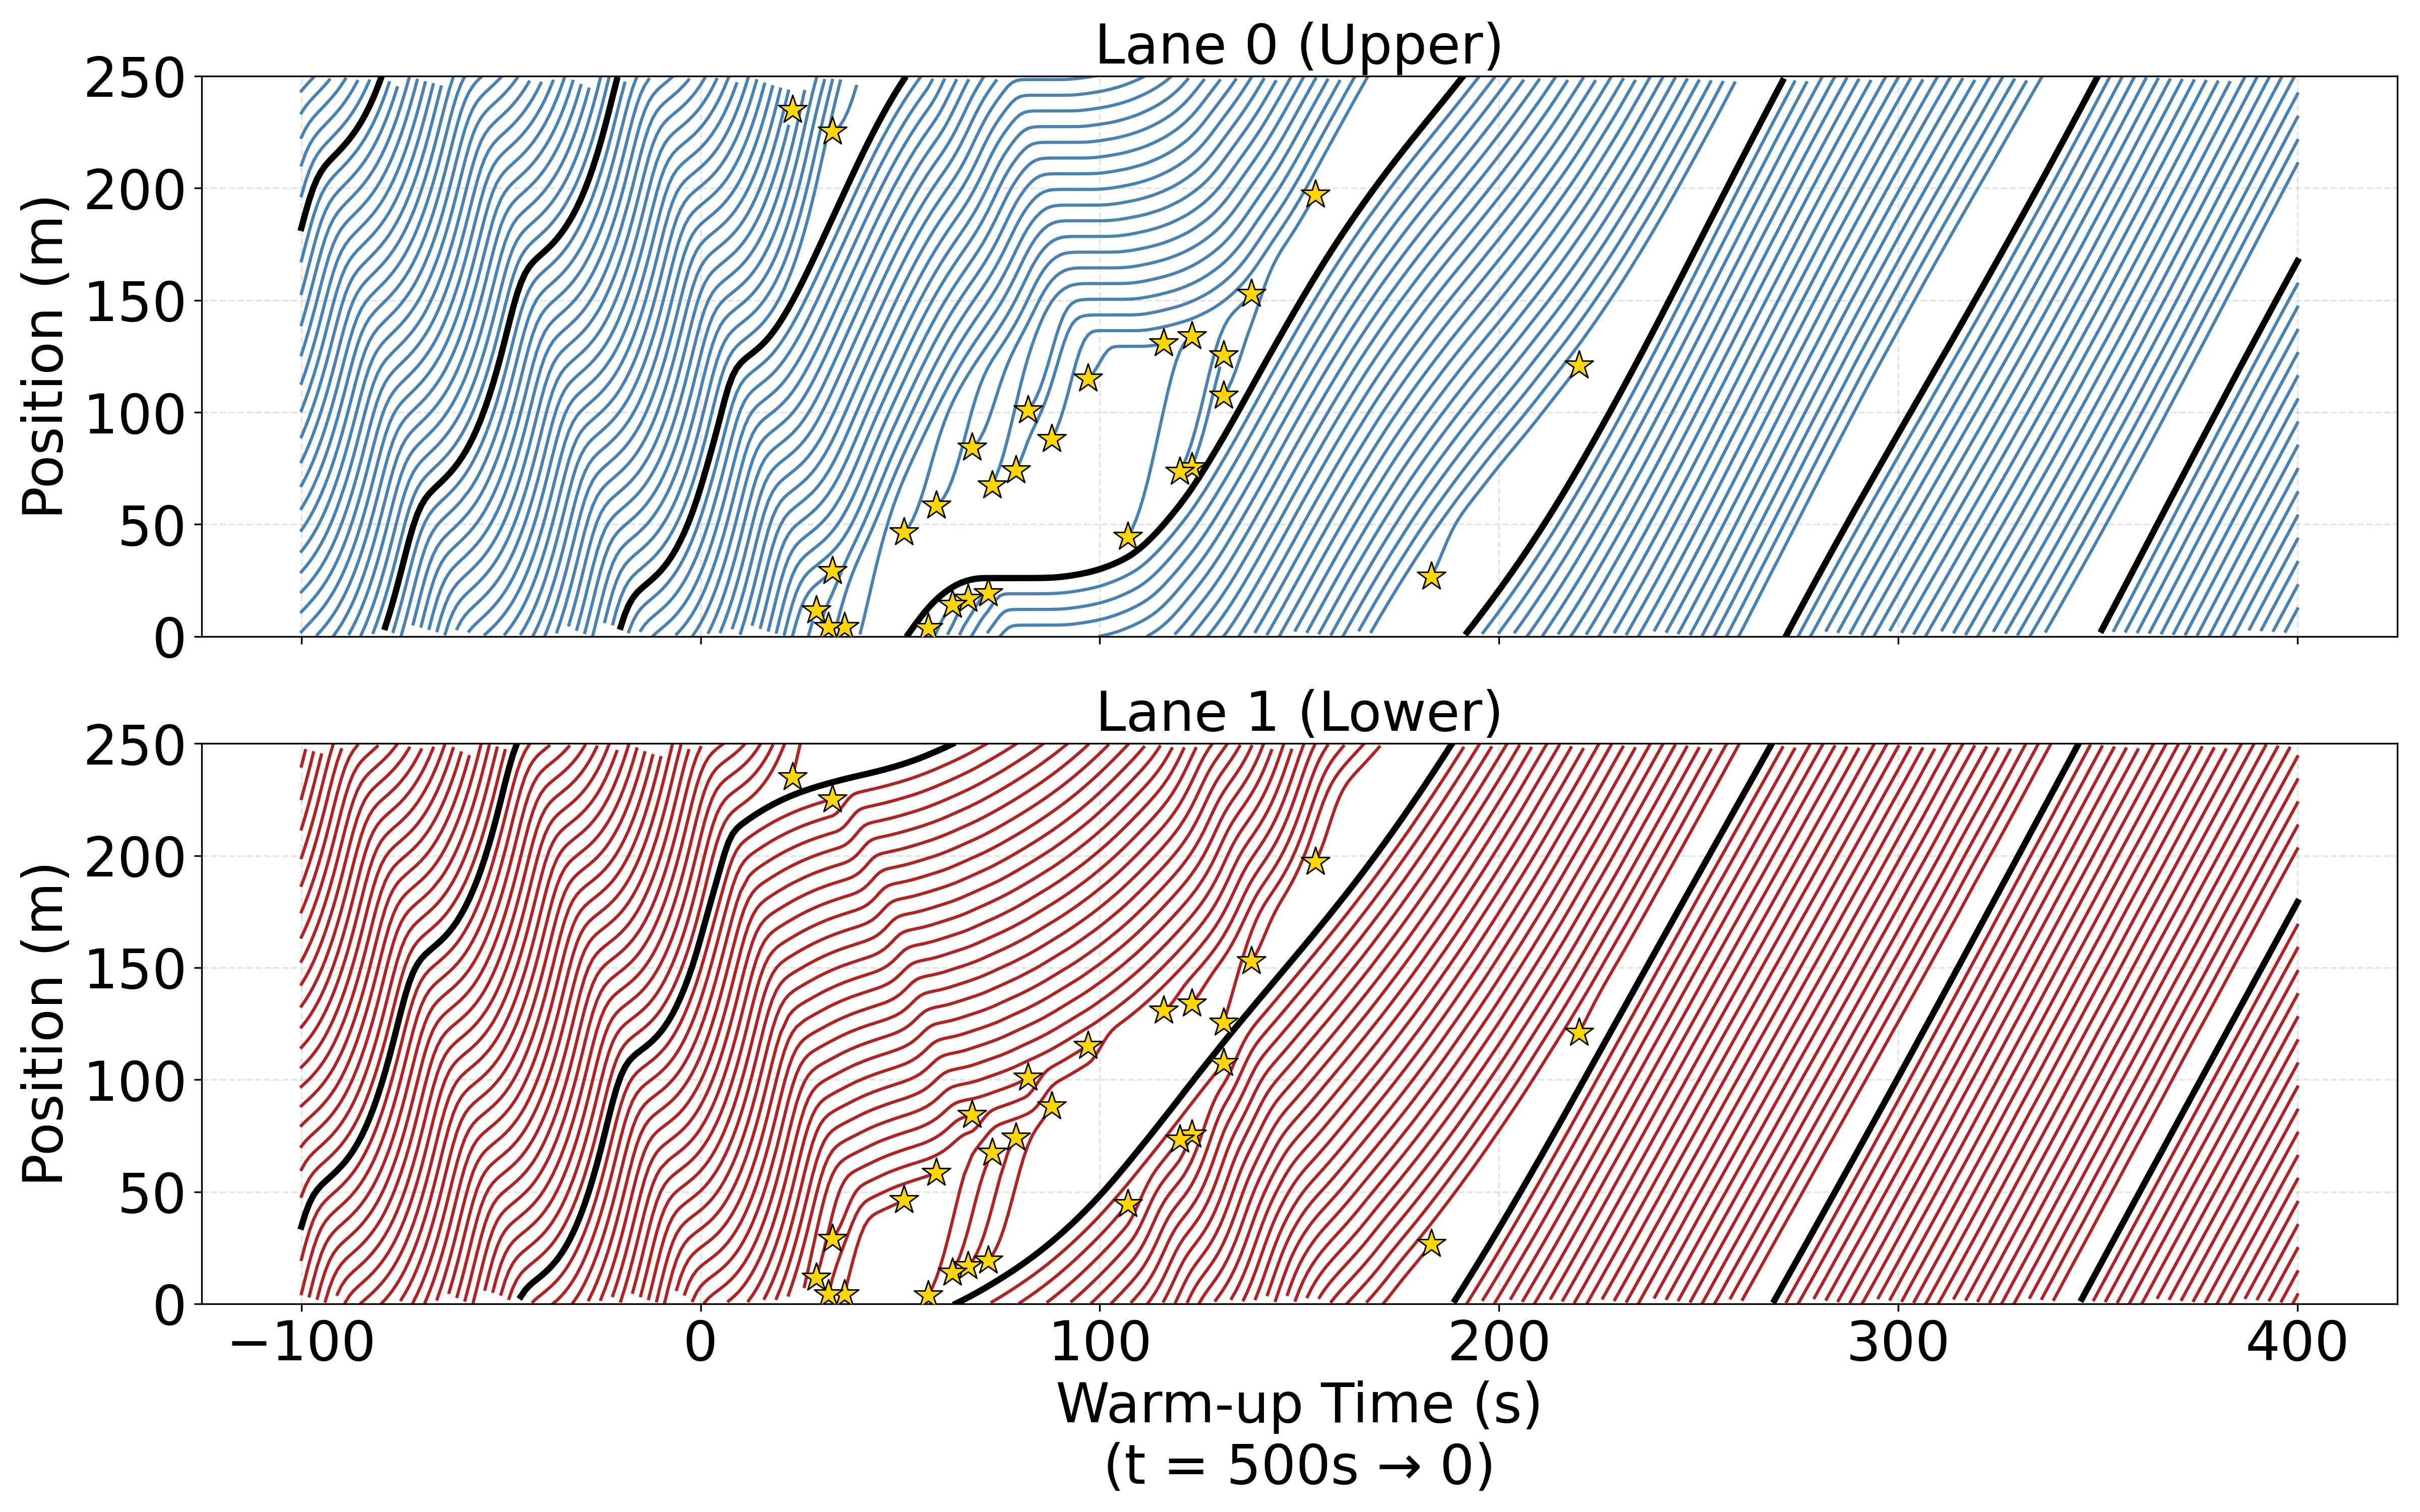
\includegraphics[width=1\linewidth]{trajectory_log_2AVCentral.png}
    \caption{Time space diagram: Cooperative RL controller governing two AVs in a double-lane ring road with lane-changing HDVs. The star markers in the figure indicate lane-changing events made by the HDVs.}
    \label{fig:2AVCEN}
\end{figure}

This coordinated pattern is discovered by the cooperative RL policy. However, this pattern also exhibits limitations. First, the paired AVs tend to form a relatively slow-moving platoon; this behavior results from the reward weights, which prioritize synchronization and stability over maintaining higher speeds. Second, while the paired structure suppresses lane-changing, the AVs often leave a considerable space ahead of them, indicating potential for improving average speed and overall traffic efficiency. The pairing mechanism can be interpreted as follows: the leading AV deliberately reduces its velocity to allow the trailing AV to close the gap, enabling the formation of a coordinated two-vehicle platoon spanning both lanes. Once formed, the pair acts as a moving bottleneck that prevents HDVs from executing lane-changing, thereby transforming the two-lane system into a single controllable virtual lane. This emergent behavior suggests that rule-based controllers inspired by this pairing mechanism may achieve similar stabilization effects with lower computational cost and greater interpretability.

\section{Rule-Based Pair-Aligned Control Strategy}\label{sec:pair}
The results presented in Section~\ref{sec:Cooperative} reveal a consistent alternating pair pattern. Inspired by it, we construct a rule-based control strategy.

\subsection{The Derived Control Design from Learning Results}
As illustrated in Fig.~\ref{fig:logic of pair}, the theoretically optimal cooperative behavior would be for both AVs to move as a tightly coupled pair—effectively functioning as a single integrated vehicle. 
Under such conditions, the original double-lane control problem can be reformulated as a single-lane cooperative control problem. 
This concept can also be generalized to multi-lane ring roads, where vehicles from different lanes form inter-lane pairs and cooperatively regulate the overall traffic flow.

\begin{figure}[t!]
    \centering
    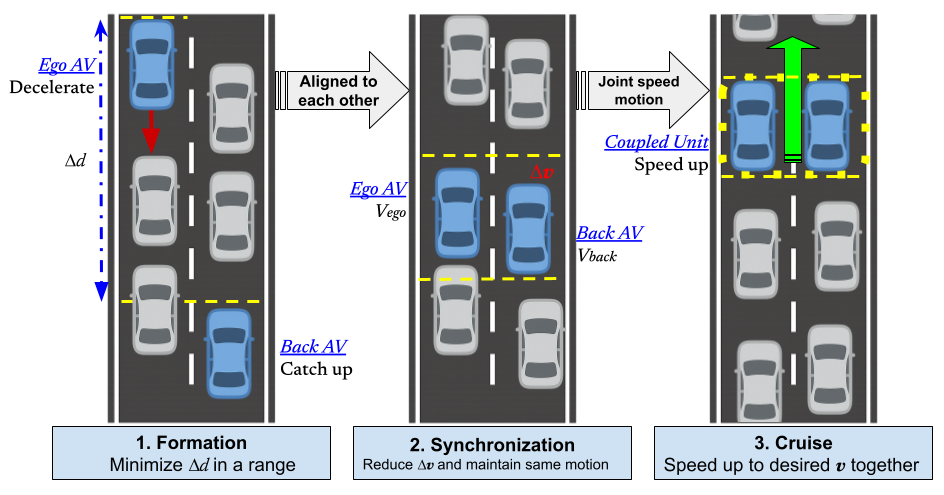
\includegraphics[width=1\linewidth]{The flowchart of paired controller.png}
    \caption{Rule-based pair-aligned control strategy}
    \label{fig:logic of pair}
\end{figure}

To enforce coherent behavior between the two AVs, we design a rule-based Pair-Aligned Control Strategy, as shown in Algorithm~\ref{alg:pair}. Let $d_p$ denote the signed longitudinal displacement between the ego vehicle and its designated
partner, and let $v$ and $v_p$ denote their respective speeds. The controller applies three hierarchical components:

1) \emph{Formation:} When $|d_p|$ exceeds a design threshold $ d_{th} $, the controller regulates longitudinal geometry through a
proportional alignment term, driving $d_p \rightarrow d_{th}$.

2) \emph{Synchronization:} If positions are aligned but a speed mismatch remains, a velocity-matching feedback term
suppresses $|v_p - v|$ until it is limited to the minimum variation $\delta_v$ and joint motion is achieved.

3) \emph{Cruise:} Once both spatial and velocity discrepancies become sufficiently small, the AV pair behaves as a single coupled unit and tracks a shared desired speed \(v^\star\) from IDM model configuration, defined as the solution to
\begin{equation*}
s_{\mathrm{eq}}^{\max} 
= \left( s_0 + v^\star \tau \right)
\left[ 1 - \left( \frac{v^\star}{v_0} \right)^{\gamma} \right]^{-1/2},
\end{equation*}
where \(s_0\), \(\tau\), \(v_0\), and \(\gamma\) are the car-following parameters.
The maximum equilibrium spacing is
\begin{equation*}
s_{\mathrm{eq}}^{\max}
= \frac{L - N s_{\min}}{N - 1},
\end{equation*}
where $N$ is the total number of vehicles on the ring, and $s_{\min}$ is the minimum safety spacing between any two consecutive vehicles. 

All acceleration commands are saturated within physical limits $a_{\max}$. This structure ensures convergence to a stable,
pairwise configuration that learning-based methods fail to maintain consistently.

\begin{algorithm}[t!]
\caption{Pair-Aligned Control Strategy}
\label{alg:pair}
\begin{algorithmic}[1]
\Require Ego state $(x, v)$; partner state $(x_p, v_p)$; control gains ($k_{\mathrm{pair}}$, $ k_{\mathrm{sync}}$, $k_v$);
\Ensure Acceleration command $a$

\State $d_p \gets (x_p - x)$ \Comment{Signed periodic displacement}

\If{$|d_p| > d_{th}$}
    \State $a \gets k_{\mathrm{pair}}\, d_p$  \Comment{Formation: spatial alignment}
\ElsIf{$|v_p - v| > \delta_v$}
    \State $a \gets k_{\mathrm{sync}} (v_p - v)$ \Comment{Synchronization}
\Else
    \State $a \gets k_v (v^\star - v)$ \Comment{Cruise: joint steady-state}
\EndIf

\State $a \gets \mathrm{clip}(a, -a_{\max}, a_{\max})$
\State \Return $a$

\end{algorithmic}
\end{algorithm}
 
\subsection{Results and Analysis}

As shown in Fig.~\ref{fig:2AVPair}, the two AVs rapidly form a paired and aligned structure across lanes and exhibit improved stabilizing performance. At the beginning of the maneuver, the leading AV decelerates sharply to allow the back AV to close the gap. During this transient phase, several HDVs attempt lane changes, but the number of such events is significantly lower compared with the purely learned RL behavior. The rule-based policy completes the pairing process more quickly, leaving fewer opportunities for HDVs to merge into the AVs’ gap.

Once the back AV successfully catches up, the pair accelerates cooperatively and reaches a higher cruising speed while preventing further lane changes. The position of AVs in both lanes are exactly same. We can see that there is fewer gaps in front of the AVs. The reduced spacing in front of the AV pair illustrates another advantage. It can minimize unnecessary gaps that HDVs could otherwise exploit. It effectively couples the two lanes into a single virtual lane, resulting in both higher stability and higher average speed. Detailed average velocity improvements, will be presented in the following section.

\begin{figure}[t!]
    \centering
    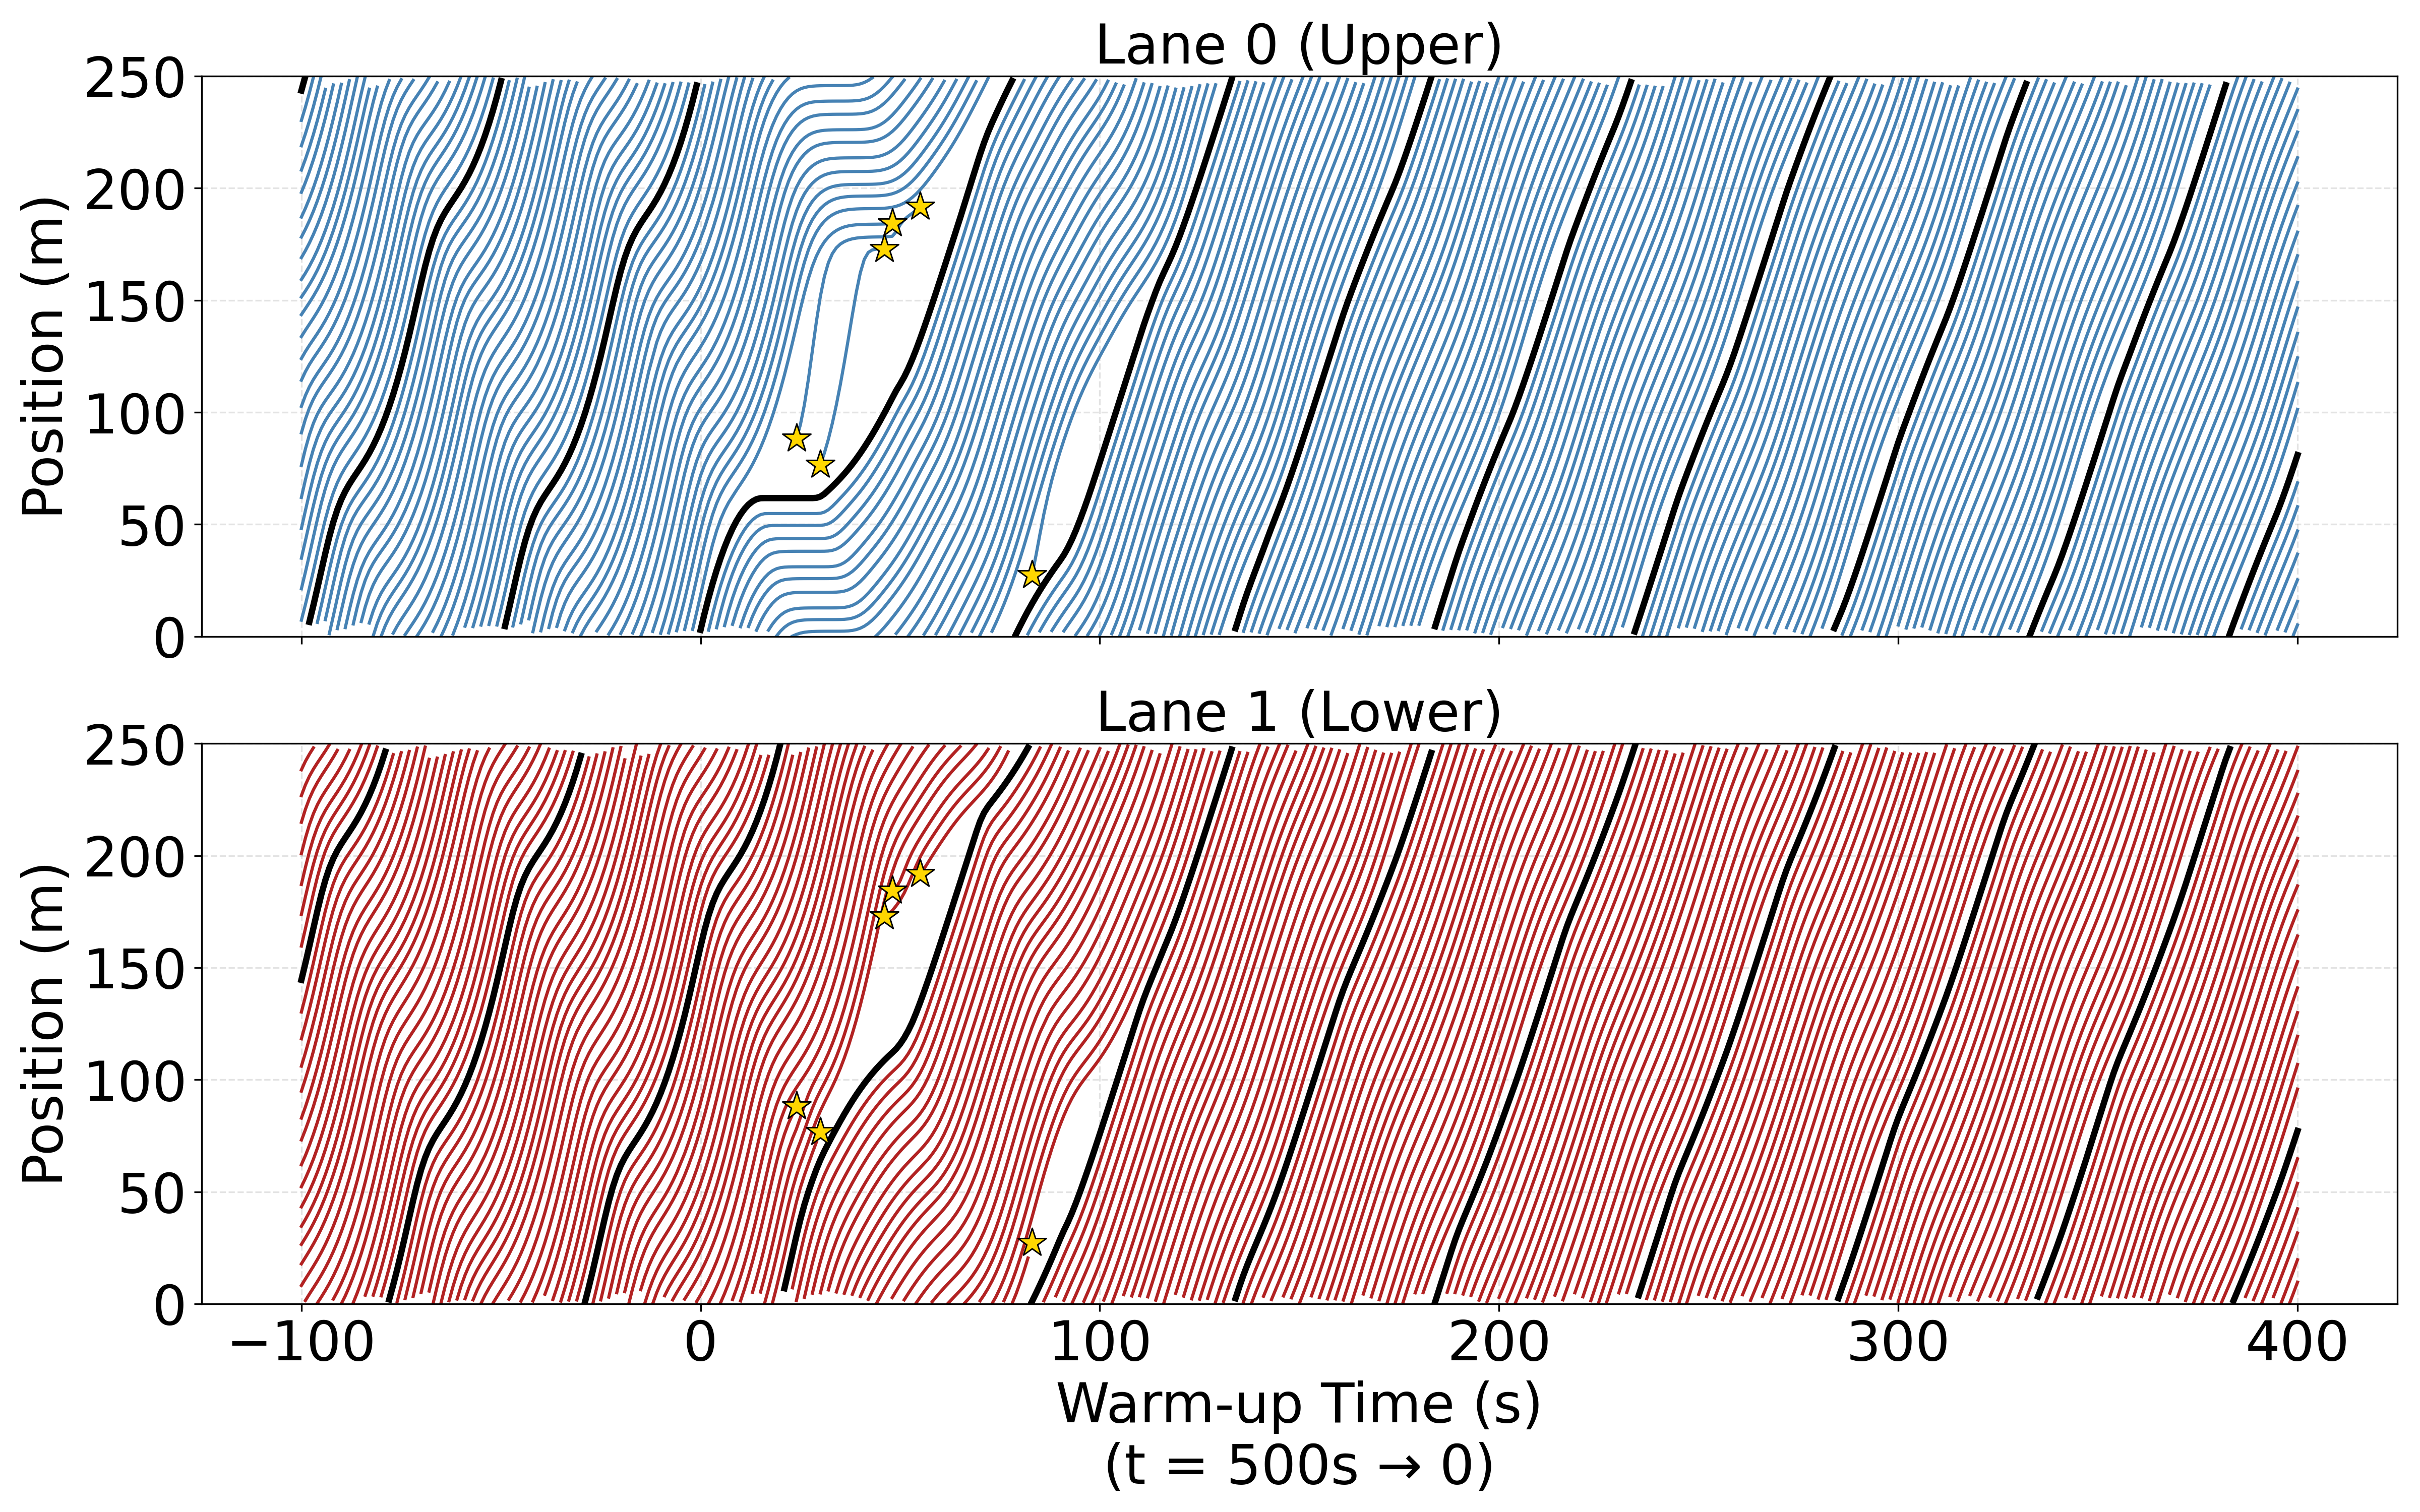
\includegraphics[width=1\linewidth]{trajectory_log_paired_controller.png}
    \caption{Time space diagram: Proposed pair-aligned rule-based controller stabilizing both lanes. The star markers in the figure indicate lane-changing events made by HDVs.}
    \label{fig:2AVPair}
\end{figure}

\section{Discussion and Comparison}
\label{sec:Discussion} 

We evaluate the rule-based controller from \citet{wu2018stabilizing} in our double-lane environment. As shown in Fig.~\ref{fig:1AVHAND}, deploying one AV under this policy stabilizes its own lane by rapidly closing gaps and maintaining a consistent speed. An early HDV lane change increases density, preventing further merging into the AV's lane. However, the adjacent lane remains highly unstable, propagating stop-and-go oscillations that increase fuel consumption and collision risks.

During the initial phase (0–50 seconds), however, at least one HDV performs a lane change, which increases local density and eliminates available gaps for subsequent merging within the AV’s lane. While this mechanism effectively prevents further lane changes in the AV’s lane, the adjacent lane continues to exhibit pronounced stop-and-go oscillations. Such oscillatory dynamics propagate throughout the network and may increase safety risks, fuel consumption, and emissions.

\begin{figure}[t!]
    \centering
    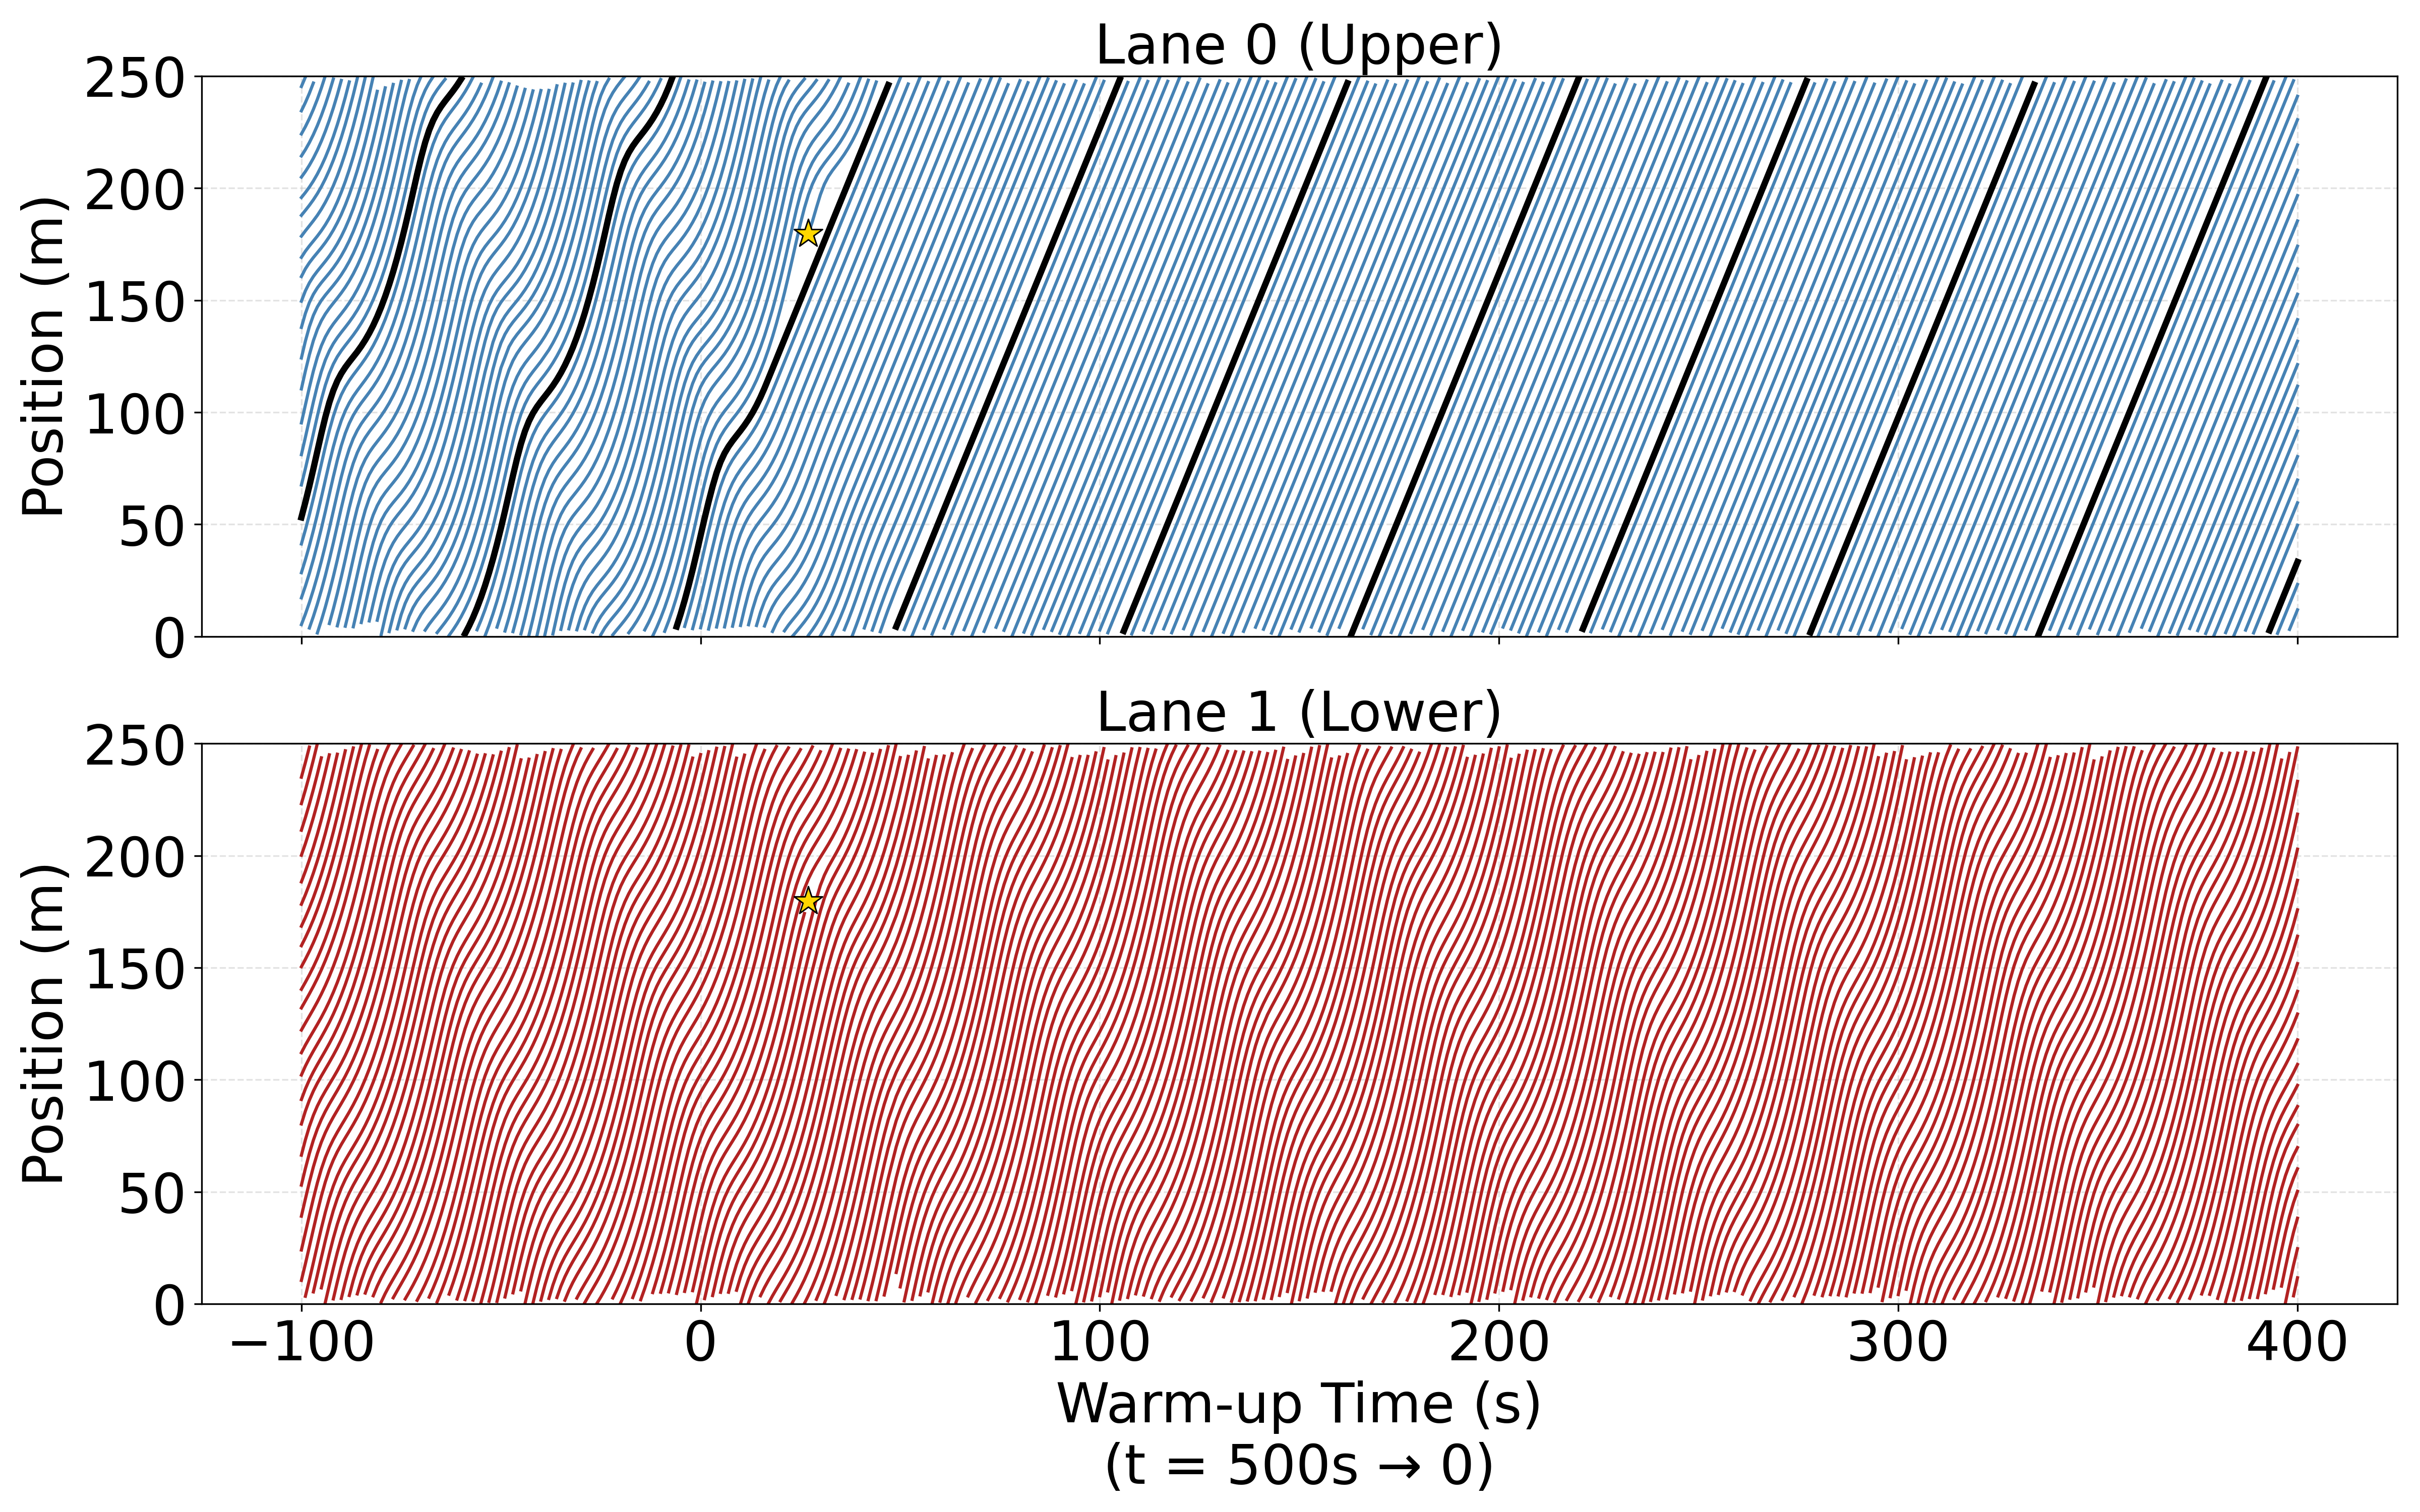
\includegraphics[width=1\linewidth]{trajectory_log_handcraft.png}
    \caption{Time space diagram: Single-lane stabilization controller applied to one AV in a two-lane ring with lane-changing HDVs. The star markers in the figure indicate lane-changing events made by HDVs.}
    \label{fig:1AVHAND}
\end{figure}

Because the controller was originally designed for a single-lane setting without explicit lateral considerations, we further examine its performance when two AVs—each controlled by the same rule—are placed in both lanes. As illustrated in Fig.~\ref{fig:2AVHAND}, each AV successfully stabilizes its own lane to a certain degree. Nevertheless, several limitations emerge. Although each lane individually exhibits smoother dynamics, noticeable gaps remain in front of both AVs. When two AVs operate independently across lanes, both lanes simultaneously exhibit these gap variations, unintentionally increasing the number of spatial opportunities for HDVs to switch lanes. These additional lane-changing events not only reintroduce instability but also induce unnecessary braking, increasing fuel consumption, emissions, and safety risks. Overall, while the derived controller stabilizes each lane individually, its single-lane design and lack of coordinated behavior across lanes limit its effectiveness in multi-lane environments. Considerable room for improvement remains.

\begin{figure}[h!]
    \centering
    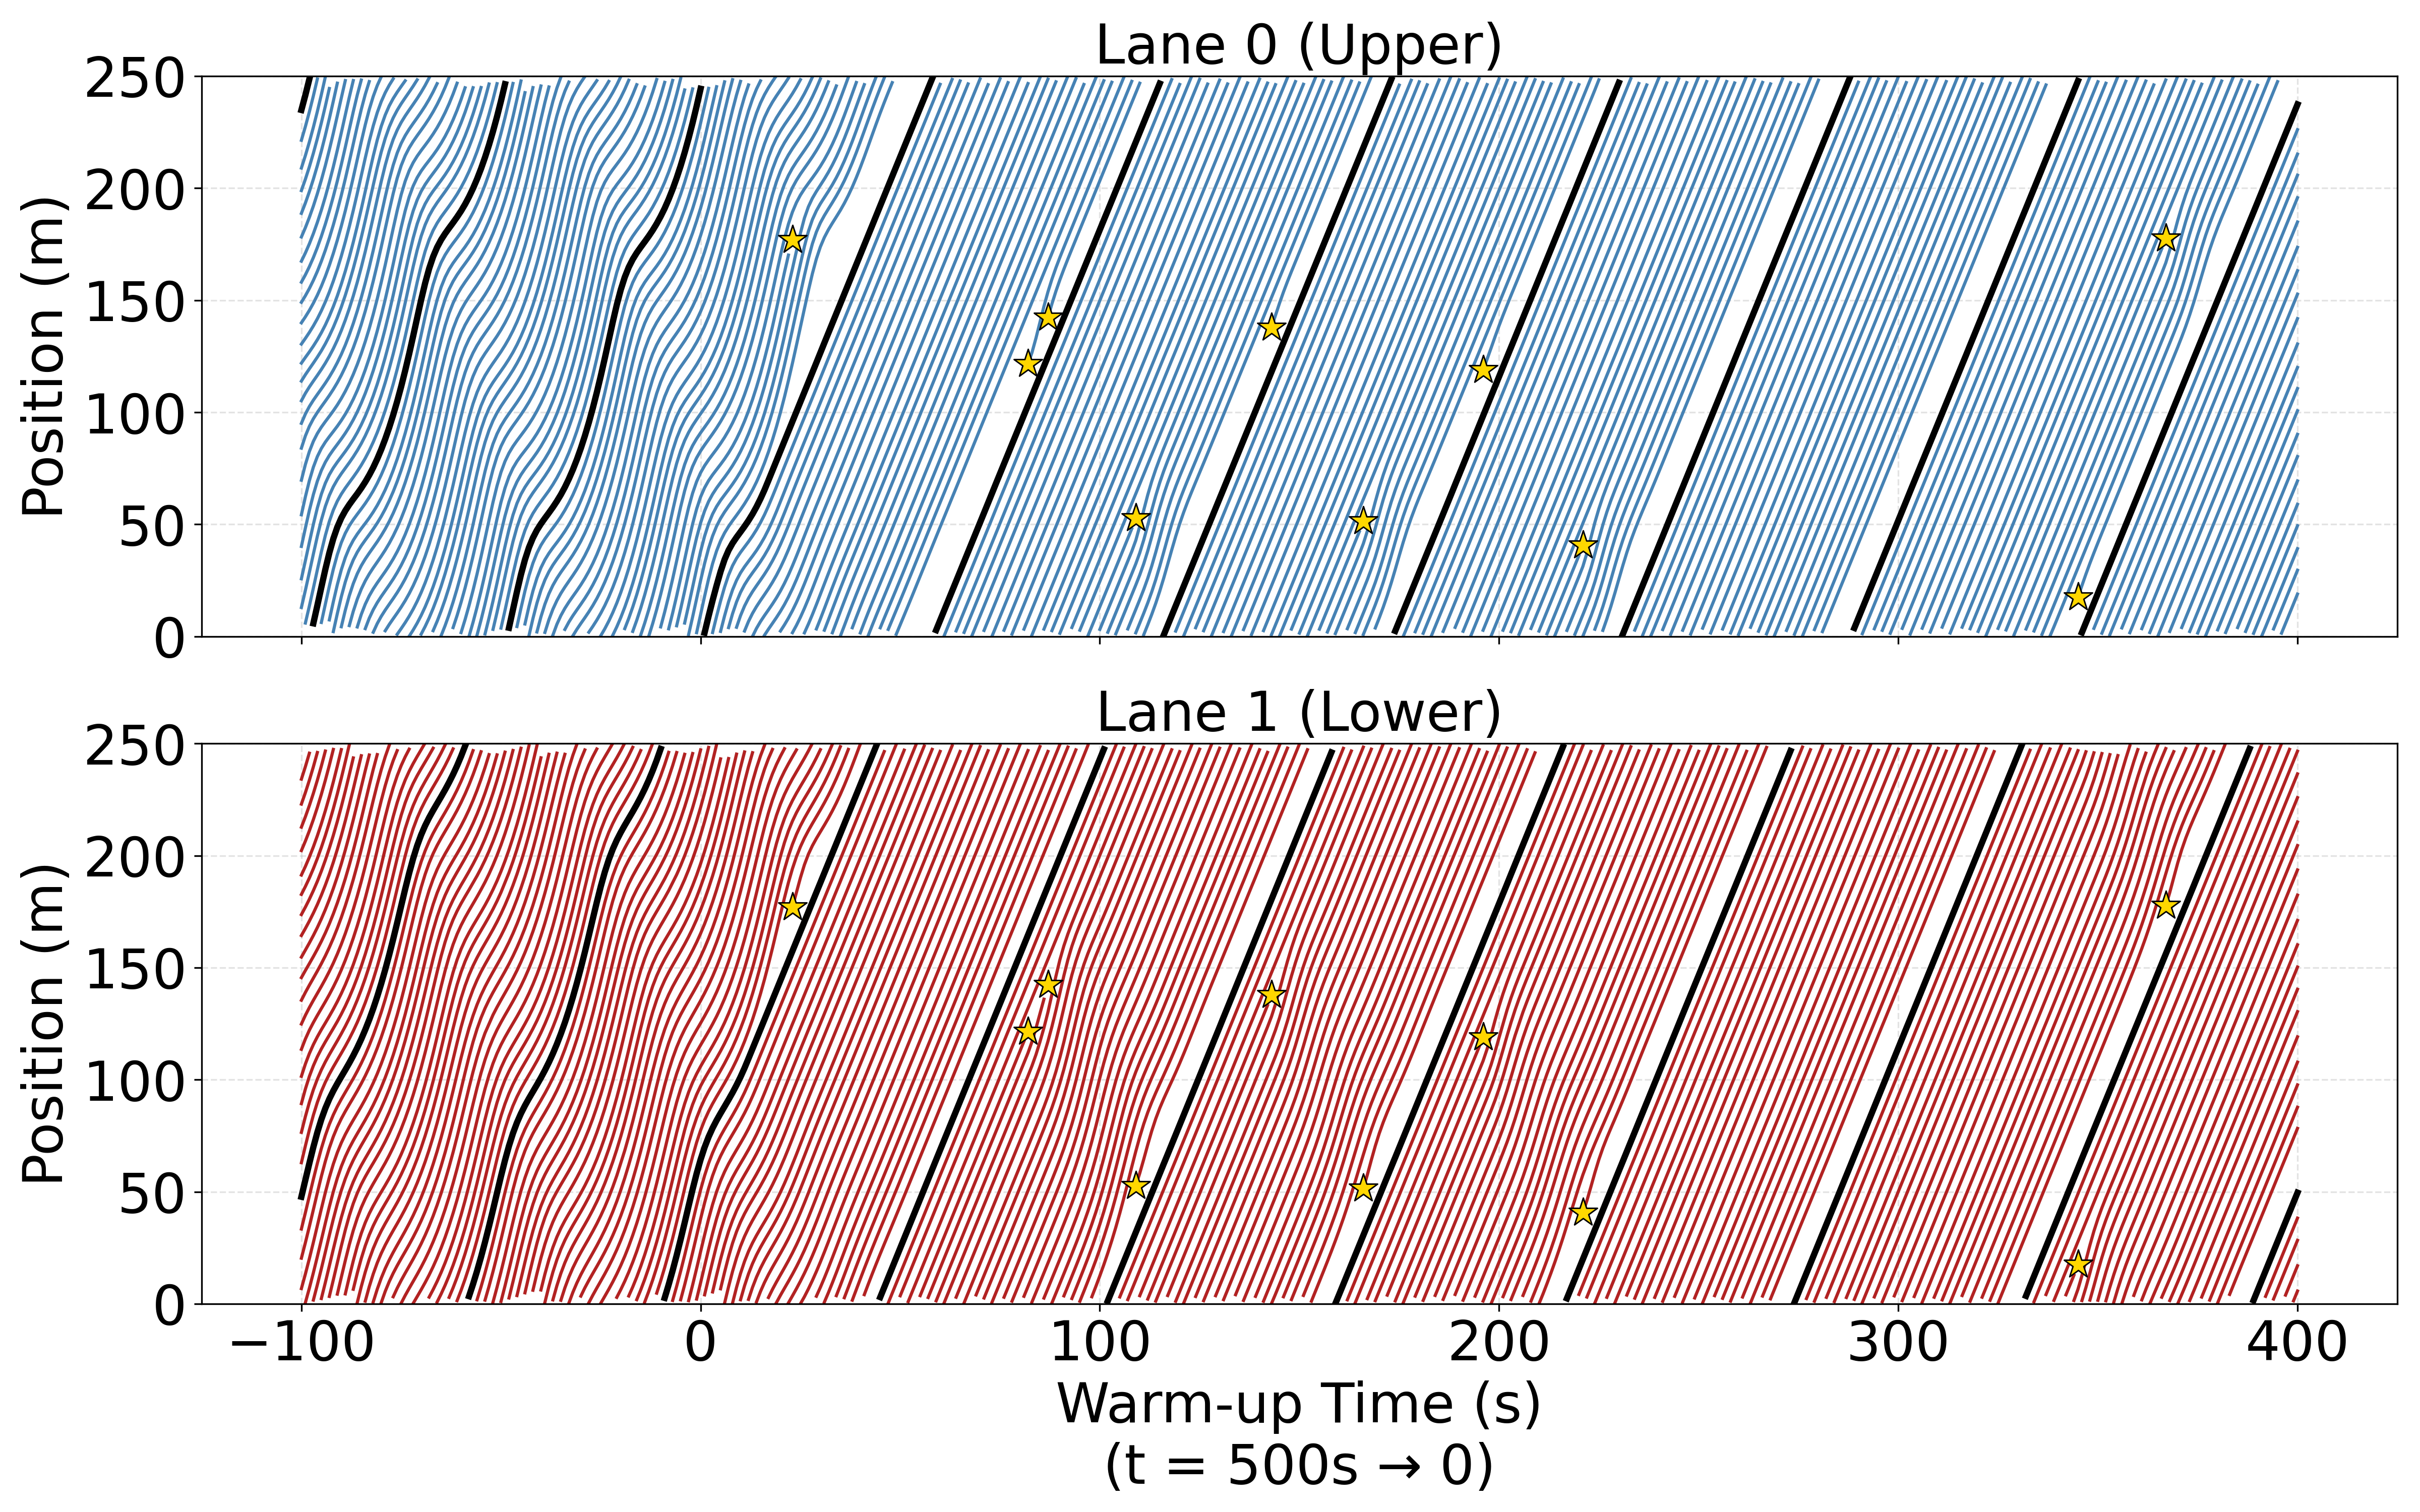
\includegraphics[width=1\linewidth]{trajectory_log_handcraft2av.png}
    \caption{Time space diagram: Independent single-lane stabilization controllers applied to two AVs across both lanes with lane-changing behavior. The star markers in the figure indicate lane-changing events made by HDVs.}
    \label{fig:2AVHAND}
\end{figure}

Figure~\ref{fig:averagespeed} summarizes the average speed across all evaluated controllers. All averages are computed over the period after $t = 500\,\text{s}$, when the controllers begin actively stabilizing the platoon.

\begin{figure}[t!]
    \centering
    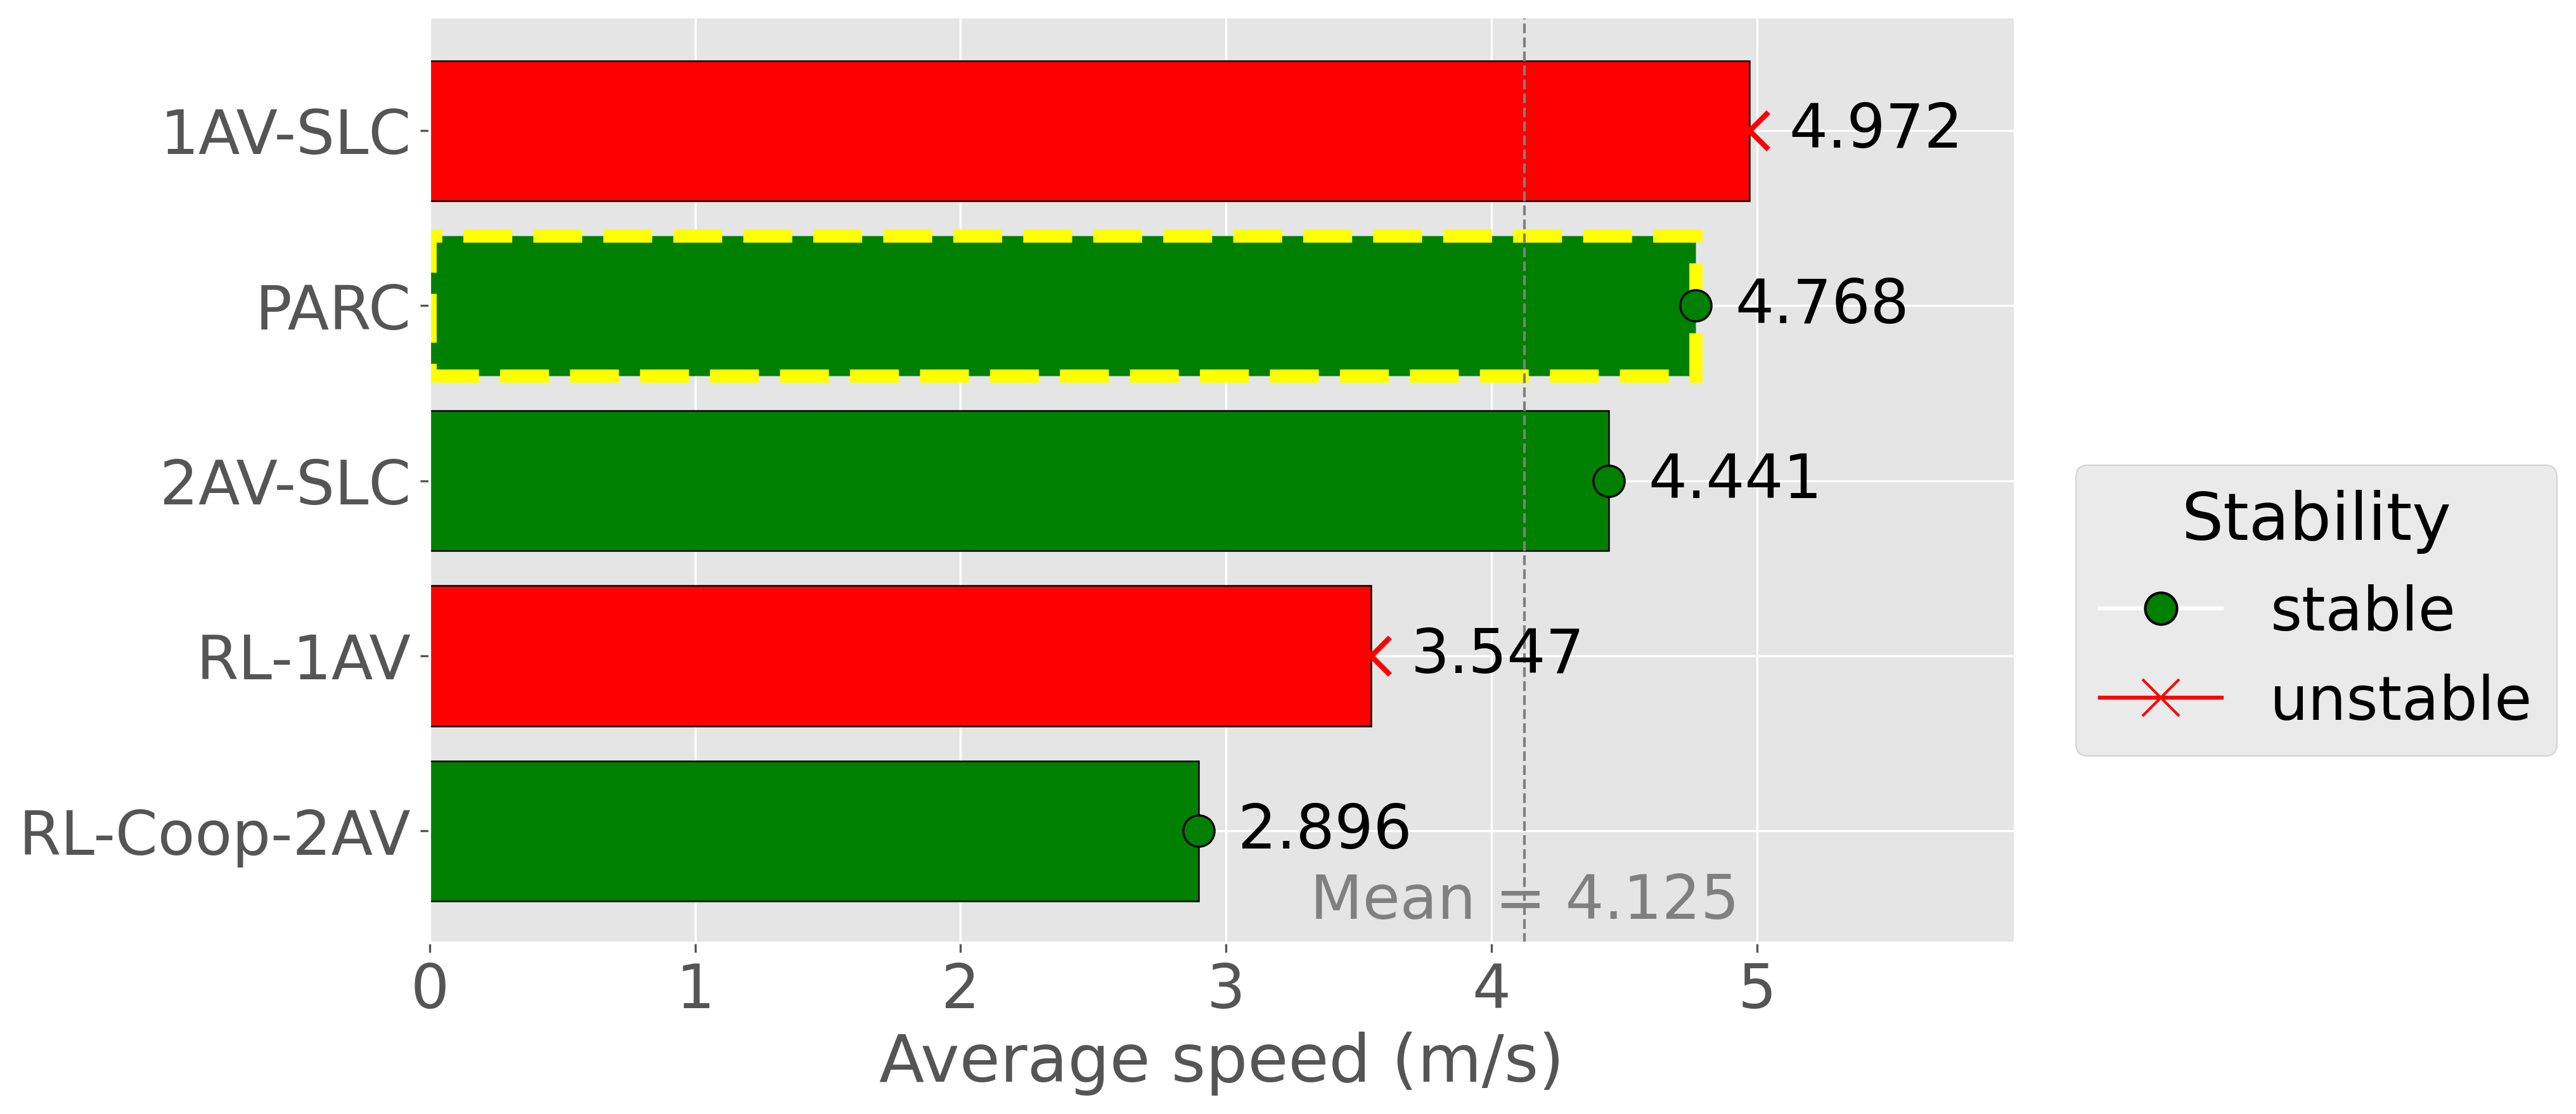
\includegraphics[width=1\linewidth]{avg_speed_comparison.png}
    \caption{Average speed under different control strategies. 
1AV-single lane controller (SLC): single-AV rule-based controller \citep{wu2018stabilizing}; 
PARC: proposed pair-aligned rule-based controller; 
2AV-SLC: two independent rule-based controllers \citep{wu2018stabilizing} applied independently to both lanes; 
RL-1AV: single-AV RL controller; 
RL-Coop-2AV: cooperative two-AV RL controller.}
    \label{fig:averagespeed}
\end{figure}

The 1AV-SLC approach achieves the highest local mean velocity ($4.972$\,m/s), but leaves the adjacent lane unstable. Deploying two independent single-lane AVs (2AV-SLC) improves overall stability but drops the average speed to $4.441$\,m/s, failing to exploit multi-lane capacity. In contrast, our proposed Pair-Aligned Rule-based Controller (PARC) simultaneously stabilizes both lanes with a competitive average speed of $4.768$\,m/s—a 7.4\% improvement over the 2AV-SLC baseline, demonstrating the advantage of coordinated cross-lane behavior. Regarding RL approaches, the single RL-controlled AV fails to stabilize mixed traffic (yielding $3.547$\,m/s). The cooperative two-AV RL policy eliminates oscillations but settles at a lower speed due to conservative reward weighting. However, its emergent pairing behavior directly inspired PARC, which successfully balances stability and efficiency. Overall, PARC effectively mitigates oscillations across both lanes while preventing the detrimental trade-offs of independent single-lane controllers.

% Overall, these findings highlight a key trade-off between efficiency and stability. Although the single-lane controller can yield high average speeds in its own lane, the remaining lane suffers from persistent stop-and-go oscillations—incurring additional fuel consumption and environmental costs. Our paired rule-based controller, inspired by cooperative RL, mitigates oscillations across both lanes while maintaining competitive average speeds. 

\section{Conclusion}
\label{sec:Conclusion}
This work demonstrates that single-lane stabilization strategies are inadequate for multi-lane mixed traffic, as cross-lane perturbations from human lane-changing fundamentally destabilize the system. Through cooperative reinforcement learning, we observed an emergent cross-lane paired formation that effectively suppresses these disturbances. Inspired by this, we proposed a rule-based pair-aligned controller that couples two lanes into a single virtual lane, reliably mitigating stop-and-go oscillations and achieving high traffic efficiency. Future work will explore decentralized multi-agent RL controllers, more realistic driver models, and diverse traffic scenarios.

\balance
\scriptsize
\bibliography{ifacconf}

  
\end{document}